%  LaTeX support: latex@mdpi.com 
%  For support, please attach all files needed for compiling as well as the log file, and specify your operating system, LaTeX version, and LaTeX editor.

%=================================================================
\documentclass[biomimetics,article,submit,pdftex,moreauthors]{Definitions/mdpi} 

%\documentclass[preprints,article,submit,pdftex,moreauthors]{Definitions/mdpi} 
% For posting an early version of this manuscript as a preprint, you may use "preprints" as the journal. Changing "submit" to "accept" before posting will remove line numbers.

% Below journals will use APA reference format:
% admsci, aieduc, behavsci, businesses, econometrics, economies, education, ejihpe, famsci, games, humans, ijcs, ijfs, journalmedia, jrfm, languages, psycholint, publications, tourismhosp, youth

% Below journals will use Chicago reference format:
% arts, genealogy, histories, humanities, jintelligence, laws, literature, religions, risks, socsci

%--------------------
% Class Options:
%--------------------
%----------
% journal
%----------
% Choose between the following MDPI journals:
% accountaudit, acoustics, actuators, addictions, adhesives, admsci, adolescents, aerobiology, aerospace, agriculture, agriengineering, agrochemicals, agronomy, ai, air, algorithms, allergies, alloys, amh, analytica, analytics, anatomia, anesthres, animals, antibiotics, antibodies, antioxidants, applbiosci, appliedchem, appliedmath, appliedphys, applmech, applmicrobiol, applnano, applsci, aquacj, architecture, arm, arthropoda, arts, asc, asi, astronomy, atmosphere, atoms, audiolres, automation, axioms, bacteria, batteries, bdcc, behavsci, beverages, biochem, bioengineering, biologics, biology, biomass, biomechanics, biomed, biomedicines, biomedinformatics, biomimetics, biomolecules, biophysica, biosensors, biosphere, biotech, birds, blockchains, bloods, blsf, brainsci, breath, buildings, businesses, cancers, carbon, cardiogenetics, catalysts, cells, ceramics, challenges, chemengineering, chemistry, chemosensors, chemproc, children, chips, cimb, civileng, cleantechnol, climate, clinbioenerg, clinpract, clockssleep, cmd, cmtr, coasts, coatings, colloids, colorants, commodities, complications, compounds, computation, computers, condensedmatter, conservation, constrmater, cosmetics, covid, crops, cryo, cryptography, crystals, csmf, ctn, curroncol, cyber, dairy, data, ddc, dentistry, dermato, dermatopathology, designs, devices, diabetology, diagnostics, dietetics, digital, disabilities, diseases, diversity, dna, drones, dynamics, earth, ebj, ecm, ecologies, econometrics, economies, education, eesp, ejihpe, electricity, electrochem, electronicmat, electronics, encyclopedia, endocrines, energies, eng, engproc, ent, entomology, entropy, environments, epidemiologia, epigenomes, esa, est, famsci, fermentation, fibers, fintech, fire, fishes, fluids, foods, forecasting, forensicsci, forests, fossstud, foundations, fractalfract, fuels, future, futureinternet, futureparasites, futurepharmacol, futurephys, futuretransp, galaxies, games, gases, gastroent, gastrointestdisord, gastronomy, gels, genealogy, genes, geographies, geohazards, geomatics, geometry, geosciences, geotechnics, geriatrics, glacies, grasses, greenhealth, gucdd, hardware, hazardousmatters, healthcare, hearts, hemato, hematolrep, heritage, higheredu, highthroughput, histories, horticulturae, hospitals, humanities, humans, hydrobiology, hydrogen, hydrology, hygiene, idr, iic, ijerph, ijfs, ijgi, ijmd, ijms, ijns, ijpb, ijt, ijtm, ijtpp, ime, immuno, informatics, information, infrastructures, inorganics, insects, instruments, inventions, iot, j, jal, jcdd, jcm, jcp, jcs, jcto, jdad, jdb, jeta, jfb, jfmk, jimaging, jintelligence, jlpea, jmahp, jmmp, jmms, jmp, jmse, jne, jnt, jof, joitmc, joma, jop, jor, journalmedia, jox, jpbi, jpm, jrfm, jsan, jtaer, jvd, jzbg, kidney, kidneydial, kinasesphosphatases, knowledge, labmed, laboratories, land, languages, laws, life, lights, limnolrev, lipidology, liquids, literature, livers, logics, logistics, lubricants, lymphatics, machines, macromol, magnetism, magnetochemistry, make, marinedrugs, materials, materproc, mathematics, mca, measurements, medicina, medicines, medsci, membranes, merits, metabolites, metals, meteorology, methane, metrics, metrology, micro, microarrays, microbiolres, microelectronics, micromachines, microorganisms, microplastics, microwave, minerals, mining, mmphys, modelling, molbank, molecules, mps, msf, mti, multimedia, muscles, nanoenergyadv, nanomanufacturing, nanomaterials, ncrna, ndt, network, neuroglia, neurolint, neurosci, nitrogen, notspecified, nursrep, nutraceuticals, nutrients, obesities, oceans, ohbm, onco, oncopathology, optics, oral, organics, organoids, osteology, oxygen, parasites, parasitologia, particles, pathogens, pathophysiology, pediatrrep, pets, pharmaceuticals, pharmaceutics, pharmacoepidemiology, pharmacy, philosophies, photochem, photonics, phycology, physchem, physics, physiologia, plants, plasma, platforms, pollutants, polymers, polysaccharides, populations, poultry, powders, preprints, proceedings, processes, prosthesis, proteomes, psf, psych, psychiatryint, psychoactives, psycholint, publications, purification, quantumrep, quaternary, qubs, radiation, reactions, realestate, receptors, recycling, regeneration, religions, remotesensing, reports, reprodmed, resources, rheumato, risks, robotics, rsee, ruminants, safety, sci, scipharm, sclerosis, seeds, sensors, separations, sexes, signals, sinusitis, siuj, skins, smartcities, sna, societies, socsci, software, soilsystems, solar, solids, spectroscj, sports, standards, stats, std, stresses, surfaces, surgeries, suschem, sustainability, symmetry, synbio, systems, tae, targets, taxonomy, technologies, telecom, test, textiles, thalassrep, therapeutics, thermo, timespace, tomography, tourismhosp, toxics, toxins, transplantology, transportation, traumacare, traumas, tropicalmed, universe, urbansci, uro, vaccines, vehicles, venereology, vetsci, vibration, virtualworlds, viruses, vision, waste, water, wem, wevj, wild, wind, women, world, youth, zoonoticdis

%---------
% article
%---------
% The default type of manuscript is "article", but can be replaced by: 
% abstract, addendum, article, benchmark, book, bookreview, briefcommunication, briefreport, casereport, changes, clinicopathologicalchallenge, comment, commentary, communication, conceptpaper, conferenceproceedings, correction, conferencereport, creative, datadescriptor, discussion, entry, expressionofconcern, extendedabstract, editorial, essay, erratum, fieldguide, hypothesis, interestingimages, letter, meetingreport, monograph, newbookreceived, obituary, opinion, proceedingpaper, projectreport, reply, retraction, review, perspective, protocol, shortnote, studyprotocol, supfile, systematicreview, technicalnote, viewpoint, guidelines, registeredreport, tutorial,  giantsinurology, urologyaroundtheworld
% supfile = supplementary materials

%----------
% submit
%----------
% The class option "submit" will be changed to "accept" by the Editorial Office when the paper is accepted. This will only make changes to the frontpage (e.g., the logo of the journal will get visible), the headings, and the copyright information. Also, line numbering will be removed. Journal info and pagination for accepted papers will also be assigned by the Editorial Office.

%------------------
% moreauthors
%------------------
% If there is only one author the class option oneauthor should be used. Otherwise use the class option moreauthors.

%---------
% pdftex
%---------
% The option pdftex is for use with pdfLaTeX. Remove "pdftex" for (1) compiling with LaTeX & dvi2pdf (if eps figures are used) or for (2) compiling with XeLaTeX.

%=================================================================
% MDPI internal commands - do not modify
\firstpage{1} 
\makeatletter 
\setcounter{page}{\@firstpage} 
\makeatother
\pubvolume{1}
\issuenum{1}
\articlenumber{0}
\pubyear{2025}
\copyrightyear{2025}
%\externaleditor{Firstname Lastname} % More than 1 editor, please add `` and '' before the last editor name
\datereceived{ } 
\daterevised{ } % Comment out if no revised date
\dateaccepted{ } 
\datepublished{ } 
%\datecorrected{} % For corrected papers: "Corrected: XXX" date in the original paper.
%\dateretracted{} % For retracted papers: "Retracted: XXX" date in the original paper.
\hreflink{https://doi.org/} % If needed use \linebreak
%\doinum{}
%\pdfoutput=1 % Uncommented for upload to arXiv.org
%\CorrStatement{yes}  % For updates
%\longauthorlist{yes} % For many authors that exceed the left citation part

%=================================================================
% Add packages and commands here. The following packages are loaded in our class file: fontenc, inputenc, calc, indentfirst, fancyhdr, graphicx, epstopdf, lastpage, ifthen, float, amsmath, amssymb, lineno, setspace, enumitem, mathpazo, booktabs, titlesec, etoolbox, tabto, xcolor, colortbl, soul, multirow, microtype, tikz, totcount, changepage, attrib, upgreek, array, tabularx, pbox, ragged2e, tocloft, marginnote, marginfix, enotez, amsthm, natbib, hyperref, cleveref, scrextend, url, geometry, newfloat, caption, draftwatermark, seqsplit
% cleveref: load \crefname definitions after \begin{document}

%=================================================================
% Please use the following mathematics environments: Theorem, Lemma, Corollary, Proposition, Characterization, Property, Problem, Example, ExamplesandDefinitions, Hypothesis, Remark, Definition, Notation, Assumption
%% For proofs, please use the proof environment (the amsthm package is loaded by the MDPI class).

%=================================================================

\usepackage{subcaption}
\usepackage{algorithm}
\usepackage{algpseudocode}
\usepackage[flushleft]{threeparttable}
\usepackage{lscape}
\usepackage{makecell}
\usepackage{overpic}
\usepackage{progressbar}
\usepackage{pifont}
\usetikzlibrary{shapes.geometric, arrows.meta, positioning, fit, calc}

% CUSTOM COMMANDS
%----------------------------------------------------------
\newcommand{\greencheck}{\textcolor{green}{\ding{51}}}
\newcommand{\redx}{\textcolor{red}{\ding{55}}}

%=================================================================
% Full title of the paper (Capitalized)
\Title{A Human Intention and Motion Prediction Framework for Applications in Human-Centric Digital Twins}

% MDPI internal command: Title for citation in the left column
\TitleCitation{A Human Intention and Motion Prediction Framework for Applications in Human-Centric Digital Twins}

% Author Orchid ID: enter ID or remove command
\newcommand{\orcidauthorA}{0000-0003-0640-8026} %  Usman Asad
\newcommand{\orcidauthorB}{0000-0001-5270-6599} %  Azfar Khalid
\newcommand{\orcidauthorC}{0000-0003-2989-1559} %  Waqas Akbar Lughmani
\newcommand{\orcidauthorD}{0000-0003-4381-7435} %  Shummaila Rasheed
\newcommand{\orcidauthorE}{0000-0001-7974-4472} %  Muhammad Mahabat Khan

% Authors, for the paper (add full first names)
\Author{Usman Asad $^{1, *}$\orcidA{}, Azfar Khalid $^{2}$\orcidB{}, Waqas Akbar Lughmani $^{3}$\orcidC{} and Shummaila Rasheed $^{1}$\orcidD{}, Muhammad Mahabat Khan $^{1}$\orcidE{}}

% MDPI internal command: Authors, for metadata in PDF
\AuthorNames{Usman Asad, Azfar Khalid, Waqas Akbar Lughmani, Shummaila Rasheed, Muhammad Mahabat Khan}

% MDPI internal command: Authors, for citation in the left column (ACS style)
\AuthorCitation{Asad, U.; Khalid, A.; Lughmani, W.A.; Rasheed, S.; Khan, M.M.}

% Affiliations / Addresses
\address{%
$^{1}$ \quad Department of Mechanical Engineering, Capital University of Science and Technology, 45750, Islamabad, Pakistan; drmahabat@cust.edu.pk (M.M.K.); shummaila@cust.edu.pk (S.R.)\\
$^{2}$ \quad Digital Innovation Research Group, Department of Engineering, School of Science \& Technology, Nottingham Trent University, NG11 8NS, Nottingham, UK; azfar.khalid@ntu.ac.uk\\
$^{3}$ \quad Department of Engineering, Birmingham City University, 7XG, Birmingham, UK; waqas.lughmani@bcu.ac.uk}

% Contact information of the corresponding author
\corres{Correspondence: usman.asad@ceme.nust.edu.pk}

% Abstract
\abstract{In manufacturing settings where humans and machines collaborate, understanding and predicting human intention is crucial for enabling the seamless execution of tasks. This knowledge is the basis for creating an intelligent, symbiotic, and collaborative environment. However, current foundation models often fall short in directly anticipating complex tasks and producing contextually appropriate motion. This paper proposes a modular framework that investigates strategies for structuring task knowledge and engineering context-rich prompts to guide Vision-Language Models in understanding and predicting human intention in semi-structured environments. Our evaluation, conducted across three use cases of varying complexity, reveals a critical trade-off between prediction accuracy and latency. We demonstrate that a Rolling Context Window strategy, which uses a history of frames and the previously predicted state, achieves a strong balance of performance and efficiency. This approach significantly outperforms single-image inputs and computationally expensive in-context learning methods. Furthermore, incorporating egocentric video views yields a substantial 10.7\% performance increase in complex tasks. For short-term motion forecasting, we show that the accuracy of joint position estimates is greatly enhanced by using historical pose, gaze data, and in-context examples. Supplementary materials, videos, and the open-source implementation are available at the project website: \url{https://usmanasad88.github.io/hcdt/}}

% Keywords
\keyword{Human Digital Twin; Human Intention Prediction; Human Motion Generation; Human-Robot Collaboration; Artificial Intelligence} 

%%%%%%%%%%%%%%%%%%%%%%%%%%%%%%%%%%%%%%%%%%
\begin{document}

\section{Introduction}
The paradigm of Digital Twins, %virtual replicas of physical systems, 
has found widespread application in optimizing performance across diverse industrial sectors, including manufacturing, aerospace, and energy \citep{Andronas2021, Polini2020}.
However, conventional digital twins often prioritize technical system aspects, frequently overlooking the human element crucial for Industry 5.0.
%effective human-machine synergy.
Human-Centric Digital Twins (HCDTs) aim to address this by integrating models of human behavior, cognition, and even emotion, thereby enabling personalized and adaptive feedback to human operators \citep{Usman}. A truly effective HCDT allows the predicted intention and motion to be utilized in several ways: for real-time monitoring of operator performance, for providing semantic assistance, such as prompting the operator on the next step or flagging procedural errors, and for enabling a robotic assistant to proactively provide physical support.
Such HCDTs promise to elevate safety, efficiency, and productivity in human-machine systems, while concurrently enhancing user experience and satisfaction \citep{Umbrico2022}.
In high-mix, low-volume (HMLV) industrial contexts, traditional automation systems exhibit significant rigidity, necessitating substantial human intervention for customization and adaptation.
The advent of Machine Learning (ML), Artificial Intelligence (AI), and advanced automation technologies offers a pathway towards more flexible solutions, particularly beneficial for Small and Medium Enterprises (SMEs).
These innovations can facilitate partial automation of labor-intensive tasks or enable collaborative human-robot workflows, where humans focus on complex reasoning and dexterous manipulation, while robots manage repetitive actions \citep{Cotta2023, Sirintuna2024}.
Digital twins of these collaborative processes can further enhance skill transfer and enable remote oversight augmented by Virtual and Augmented Reality (VR/AR) \citep{Nezhad2020, Laughlin2020}.
Despite these technological strides, industrial robotics largely remains confined to pre-programmed, caged systems, with collaborative applications still in its infancy.
Recent breakthroughs in behavior cloning \citep{Mandlekar2021}, diffusion policies \citep{Chi2023}, high-fidelity simulators \citep{orbitsurgical, Liu2023}, and the proliferation of Large Language Models (LLMs) \citep{Wei2022, Fan2024} and Vision-Language Models (VLMs) \citep{li2024llava} have expanded the horizons for semantic understanding, task planning, and perception in robotic systems \citep{Singh2023, Ahn2022}.
Nevertheless, achieving robust spatial intelligence, such as forecasting detailed 3D human motion from visual inputs in partially structured settings, remains an important challenge.
Humans possess an innate ability to predict future actions by synthesizing contextual clues, prior knowledge, and spatial reasoning.
For instance, when a person glances at an empty cup and then starts to stand, it indicates a likely intent to get a drink.

Current AI systems are approaching a semantic understanding of such scenarios, but translating this understanding into accurate 3D motion prediction remains an open problem. This predictive capability is paramount for robots to transition from reactive assistance to smart collaboration. To address this challenge, this paper proposes a modular and scalable framework that utilizes Vision-Language Models (VLMs) with motion diffusion techniques to predict human intent and generate plausible future human motion in semi-structured environments. Instead of pursuing the end-to-end training, the approach emphasizes the integration of existing, pre-trained perception and reasoning modules. This design philosophy not only makes the system more practical for SMEs with limited resources but also ensures adaptability, as overall performance can improve with advancements in individual modules. To validate this framework, three use case scenarios with varying levels of complexity are utilized. These include scenarios from existing datasets such as HaVID \citep{havid} and EgoExo4D \citep{egoexo}. This provides a systematic evaluation of the framework's ability to perform context-driven, intention-aware motion prediction. The remainder of this paper is structured as follows: Section \ref{sec:related_work} reviews related research. Section \ref{sec:methodology} details the proposed framework. Section \ref{sec:experimental_validation} presents the validation approach and experimental results. Finally, Section \ref{sec:discussion_conclusion} discusses the implications of this work and outlines future directions.

\section{Background and Related Work} \label{sec:related_work}

The endeavor to create proactive robotic assistants capable of anticipating human needs and actions draws upon several interconnected research areas.
This section reviews pertinent work in human intent prediction for Human-Robot Collaboration (HRC), AI-driven human motion generation, the role of LLMs in robotics, and the critical aspect of datasets available for these tasks.
\subsection{Human Intent Prediction for Collaborative Environments}
Anticipating human intent is pivotal to enhancing safety, security, ergonomics, and effective collaboration in Industry 5.0. Early work often focused on trajectory prediction in constrained scenarios \citep{Huang2021}. More recent approaches have sought to infer higher-level goals.
For instance, Huang et al. \citep{Huang2022} proposed a hierarchical intention-tracking framework for assembly tasks, utilizing OpenPose and Kalman filtering to track wrist positions and infer both high-level task goals and low-level current actions.
Similarly, Mangin et al. \citep{Mangin2022} developed hierarchical planners that infer human goals using partially observable Markov decision processes for procedural tasks.
These methods underscore the importance of structured task understanding.

The integration of richer sensory data and more sophisticated AI models is an ongoing trend.
Zhong et al. \citep{Zhong2024} introduced a framework for human-robot handover tasks that fuses a hierarchical human digital twin with deep domain adaptation, leveraging spatio-temporal graph convolutional networks.
Ding et al. \citep{Ding2024} proposed a dynamic scenario-enhanced network for predicting stochastic motions in customized assembly tasks, highlighting the need to handle variability.
The use of egocentric data has also gained traction, with works like Mascaro et al.
\citep{Mascaro2022} developing intention-conditioned hierarchical architectures for long-term action anticipation based on the Ego4D dataset \citep{Grauman2021}.
However, many existing methods focus on recognizing intent from past actions rather than proactively forecasting future motion linked to that intent. They also often lack robust integration with real-time simulation for physical plausibility.
\subsection{AI-Driven Virtual Human Motion Generation}
Generating realistic and controllable human motion is a long-standing challenge in computer graphics and AI. The field has historically relied on motion capture (MoCap) datasets, which provide high-fidelity kinematic data for a wide range of human activities. A significant advancement was the creation of large-scale datasets pairing MoCap data with natural language descriptions, such as HumanML3D \citep{Guo_2022_CVPR}. Pioneering works like Adversarial Motion Priors (AMP) \citep{2021-TOG-AMP, Peng2021} trained reinforcement learning (RL) policies to perform tasks while using a discriminator to ensure the resulting motions were realistic and stylistically similar to MoCap examples. This was extended by models like Adversarial Skill Embeddings (ASE) \citep{2022-TOG-ASE} and Conditional Adversarial Latent Models (CALM) \citep{Tessler2023}, which focused on learning a low-dimensional latent space that could be sampled to direct a character's behavior.

With the advent of kinematic diffusion models, Human Motion Diffusion Model (MDM) \citep{tevet2023human}  demonstrated a remarkable ability to generate complex motions from text prompts alone. However, these purely kinematic approaches often produce physically implausible motions with artifacts such as foot-sliding, floating, and ground penetration because they lack physical grounding. PhysDiff \citep{Yuan2023} introduced a novel physics-guided approach that incorporates a physics simulator directly into the diffusion process, thereby correcting the motion to adhere to physical constraints.

Recent work has focused on creating unified controllers that combine the strengths of generative models with the realism of physics-based simulation for more interactive and multi-modal control. MaskedMimic \citep{tessler2024masked} presents a unified framework that formulates physics-based character control as a versatile motion inpainting problem. It trains a single controller to synthesize full-body, physically plausible motions from partial or "masked" inputs, which can include any combination of target joint positions, text commands, or object interactions. Another state-of-the-art approach, CLoSD \citep{tevet2024closd}, closes the loop between motion planning and execution. It uses a real-time, autoregressive Diffusion Planner (DiP) to generate kinematic motion plans on-the-fly, which are then executed by a robust RL-based tracking controller in a physics simulator.  However, these MoCap-based methods often lack the rich scene-interaction context necessary for robustly forecasting actions in unstructured, real-world environments.

\subsection{The Role of LLMs in Intelligent Robots}
The advent of LLMs has opened new avenues for enhancing the semantic understanding and planning capabilities of robotic systems.
LLMs can parse natural language instructions, reason about task goals, and even generate plans or code snippets for robotic execution \citep{Fan2024, Singh2023}.
For instance, SayCan \citep{Ahn2022} demonstrated how LLMs can propose high-level actions grounded by pretrained robotic skills.
Singh et al. \citep{Singh2023} developed ProgPrompt using programmatic LLM prompts to generate executable plans. Ha et al.
\citep{Ha2023} explored using LLMs to guide high-level planning for data collection and then distilling this into visuomotor policies.
Further, efforts like "Asking Before Action" by Chen et al. \citep{Chen2023} empower LLM agents to proactively seek information.
These works highlight LLMs' potential in interpreting complex instructions and decomposing them into actionable steps. However, they are primarily designed to interpret high-level commands and map them to a robot's own action space. They are not inherently structured to analyze a continuous stream of human motion and environmental context to proactively predict a human's future intent and generate a corresponding, physically plausible motion trajectory, which is the central focus of our work.
The Magentic-One framework \citep{magentic} showcases the potential of multi-agent systems driven by LLMs for complex task solving.
However, grounding LLM outputs in the physical world, ensuring feasibility, and integrating them with continuous motion generation remain active research areas.
\subsection{Datasets for Human Motion and Intent}
The development of robust models for intention-based motion generation is intrinsically linked to the availability of suitable datasets.
Motion capture (MoCap) datasets, such as AMASS \citep{AMASS} and HumanML3D \citep{Guo_2022_CVPR}, offer precise 3D human kinematics.
These datasets are invaluable for learning the fundamental dynamics and stylistic nuances of human movement.
However, they are typically recorded in controlled laboratory settings and often lack the rich object interactions and complex environmental context necessary for inferring high-level human intent.
While some, like the KIT Motion-Language dataset \citep{Plappert2016}, pair motion with textual descriptions, these descriptions usually label the overt action rather than the underlying intent or the broader task goal.
Consequently, their utility for training models that predict intent from a wider range of cues is limited.
Conversely, video-based datasets such as Ego4D \citep{Grauman2021}, EgoExo4D \citep{egoexo}, Assembly101 \citep{assembly101}, and HaVID \citep{havid} provide a wealth of visual context, capturing humans performing tasks in more natural, often cluttered, environments.
Ego4D, with its extensive collection of egocentric video, offers a first-person perspective on daily activities.
EgoExo4D complements this with synchronized exocentric views, providing a more holistic understanding of human actions and interactions within a scene.
Assembly101 focuses specifically on procedural assembly tasks, offering structured sequences of actions.
HaVID \citep{havid} contributes a dataset focused on human assembly with an emphasis on comprehensive knowledge understanding, including granular action annotations.
These datasets are more conducive to understanding human-object interactions and inferring short-term goals or intents from visual cues and task progression.
However, extracting precise, full-body 3D human motion comparable to MoCap quality from these "in-the-wild" videos remains a significant challenge, often relying on human pose estimation using methods like Multi-HMR \citep{multi-hmr2024}.

This reveals a critical gap in current research: the lack of a unified framework capable of synthesizing rich, multi-modal human observations, such as visual data, pose dynamics, and gaze, with formal task knowledge. A bridge is missing to connect the semantic, long-term understanding derived from these inputs with a physically plausible forecast of future movements.

This work directly addresses this gap by proposing a novel, modular framework that creates a pipeline from these specific multimodal inputs to semantic intent prediction and, ultimately, to context-aware motion synthesis. This approach provides a solution for proactive forecasting, a necessary capability for enabling symbiotic human-machine systems in complex environments.

\section{Proposed Framework}
%for Human Intent and Motion Forecasting
\label{sec:methodology}

A modular framework is proposed to enable intelligent HRC by predicting human intention and future pose. This methodology is designed to bridge the gap between short-term motion forecasting and long-term action planning, ensuring predictions are both physically plausible and contextually appropriate.

% Formally, the predictive challenge is to process a stream of multimodal data to predict human intention and motion. 
Let the input at any given time $t$ consist of a history of video frames $\mathcal{V} = \{I_k\}_{k=1}^t$, extracted human poses $\mathcal{P} = \{P_k\}_{k=1}^t$, and static, high-level task knowledge $\mathcal{C}_{task}$. The framework, represented by a function $\mathcal{F}$, processes this context to give three outputs: the predicted task state $S_t$, a forecast of future hand positions $\hat{H}_{t+\Delta t} = ( (x_l, y_l), (x_r, y_r) )$, for a time horizon $\Delta t$, and a full-body 3D motion trajectory $\hat{M}_{t_i} = \{\hat{x}_{t_i+1}, \ldots, \hat{x}_{t_i+N_{\text{pred}}}\}$.

The proposed framework, as shown in Figure \ref{fig:pic1} has three primary modules: a Perception and Scene Representation Module that processes raw visual data; an AI-Driven Reasoning and Prediction Module that infers task state and forecasts future actions; and a downstream Motion Generation Module that synthesizes full-body 3D motion. The specific functions of each of these modules are detailed in Sections \ref{sec:sceneunderstanding} through \ref{sec:motiongeneration}. This modularity allows for individual modules to be upgraded as technology advances. While the framework provides the necessary predictive outputs for a complete Human-Centric Digital Twin (HCDT), the implementation of feedback and physical assistance mechanisms is designated as future work.

% Figure 1
\begin{figure}[H]
  \centering
    
\includegraphics[width=\textwidth]{Framework.png}
    \caption{Conceptual overview of the proposed modular framework for Human Intention Prediction based Motion Generation. Information flows from the physical system through the perception and reasoning modules to generate a final motion prediction.} 
    \label{fig:pic1}
\end{figure}

\subsection{Perception and Scene Representation}
\label{sec:sceneunderstanding}
% \subsubsection{Human Pose Representation.}
The framework adopts the Skinned Multi-Person Linear Model with Extensions (SMPL-X) \citep{SMPL-X:2019}, which provides a parametric model for body shape $\boldsymbol{\beta}$, pose $\boldsymbol{\theta}$, and expressive hand and face parameters $\boldsymbol{\psi}$. To obtain the pose parameters from monocular RGB video, we employ World-Grounded Human Motion Recovery via Gravity-View Coordinates (GVHMR) \citep{multi-hmr2024, gvhmr}. GVHMR reconstructs human pose in a global, gravity-aligned coordinate system. For kinematic motion generation, the SMPL-X poses are subsequently converted into the representation utilized by HumanML3D \citep{Guo_2022_CVPR}.
This format captures frame-relative information such as root angular and linear velocities ($\dot{r}_a, \dot{r}_x, \dot{r}_z$), root height ($r_y$), and local joint positions, rotations, and velocities ($j_p, j_r, j_v$), along with foot contact features ($f$).
This relative encoding facilitates the generation of smooth and continuous motions.

% \subsubsection{3D Scene Grounding.}
Additionally, this module is required to convert the VLM's 2D predictions into 3D world coordinates. The proposed method extracts the global 3D coordinates of points of interest (POIs) from monocular video by combining world-frame human pose reconstruction results and metric depth estimation, using models like Unik3D \citep{unik3d}. By leveraging the global-to-camera transformation $R_{wc}, \mathbf{t}_{wc}$ provided by GVHMR, camera-centric 3D points $\mathbf{x}_c$ can be transformed into a consistent world frame via $\mathbf{x}_w = R_{wc}^\top (\mathbf{x}_c - \mathbf{t}_{wc})$. This allows any POI, such as a tool or a predicted hand location, to be localized in the global reference frame. For specialized applications requiring different or higher-precision grounding, this module can be extended to incorporate other engineered approaches, such as processing fiducial markers.

This module also incorporates human gaze target analysis, which provides a strong cue for immediate intent. A change in the operator's gaze target is a good indicator of a change in intention, and the location of the gaze target often correlates with the area or object the operator intends to interact with next. Techniques like Gaze-LLE \citep{ryan2024gazelle} can be employed for gaze target tracking to further enrich the context provided to the reasoning and intent prediction module.


\subsection{AI-Driven Reasoning and Intent Prediction}
This module serves as the cognitive core of the framework. The integration of VLMs for high-level reasoning about tasks and intent requires appropriate data structures. Task dependencies are modeled using formalisms like Directed Acyclic Graphs (DAGs), which define the valid sequence of actions and states. Alternative formalisms, such as Planning Domain Definition Language (PDDL) \citep{Singh2023}, Knowledge Graphs (KGs), or Behavior Trees (BTs) \citep{Ahn2022, IEEE-Knowledgebased2021}, can also be integrated. For any use case, a common operational flow is followed. Initially, task-specific knowledge, such as assembly instructions or procedural steps, or an example video, is provided to the system. This involves a collaborative effort where an AI model generates an initial draft of a task representation (i.e., an action graph and state schema), which is then refined by human experts. This task representation, encompassing the overall goal, a mechanism for state tracking, a decomposition into smaller actions, and their dependencies, forms a critical part of the context.

The prediction process follows a two-phase approach. The VLM analyzes video frames and appropriate context from the perception module, as well as the task graph, to first output an updated Task State in a structured JSON format. Here, the system identifies the steps completed, in progress, available, and the immediate next step. In the second phase, the VLM uses this updated task context and multimodal data from the perception module, to forecast the exact pixel coordinates (\texttt{x, y}) for both of the operator's hands at a future time horizon. This two-phase pipeline is illustrated in Figure \ref{fig:prediction_pipeline}. This two-phase approach is crucial because it decouples long-horizon semantic reasoning about the overall task from short-horizon spatiotemporal forecasting of immediate motion, allowing each phase to be optimized with the most relevant context. In this module, various prompting strategies are investigated to optimize the VLM's predictive accuracy, which are discussed in Section \ref{sec:eval}.

% Figure 2
\begin{figure}[H]   
\subfloat[\centering]{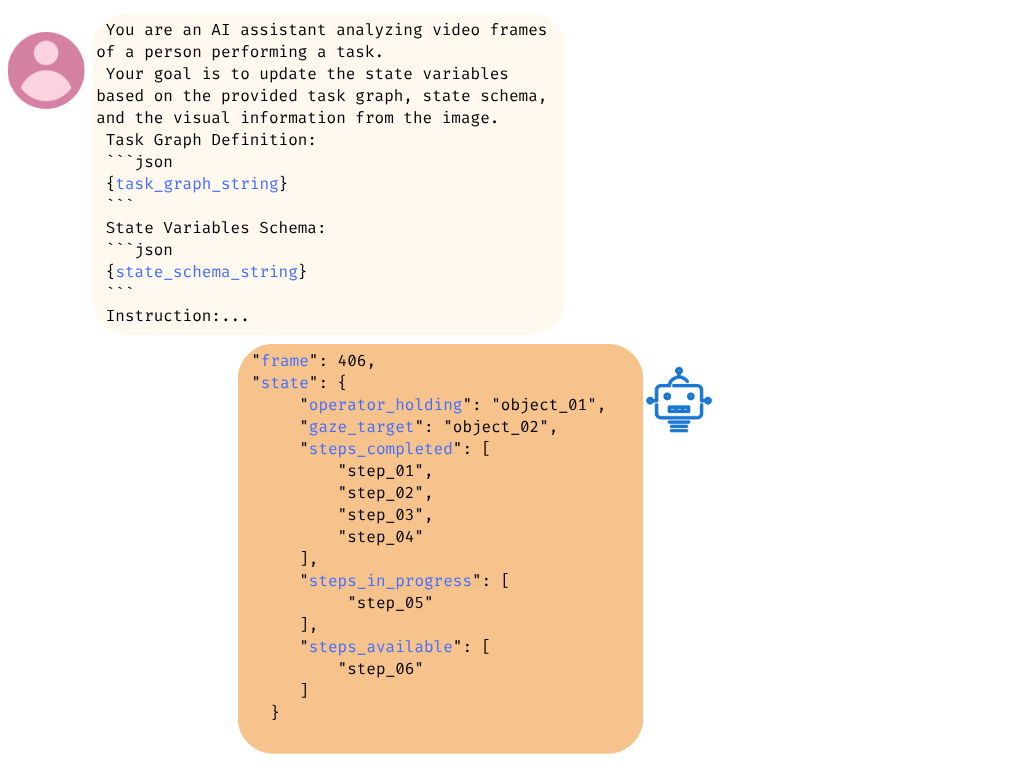
\includegraphics[width=0.48\textwidth, trim=5 0 235pt 0, clip]{s5.png}\label{fig:task_state_prediction}}
    \hfill
\subfloat[\centering]{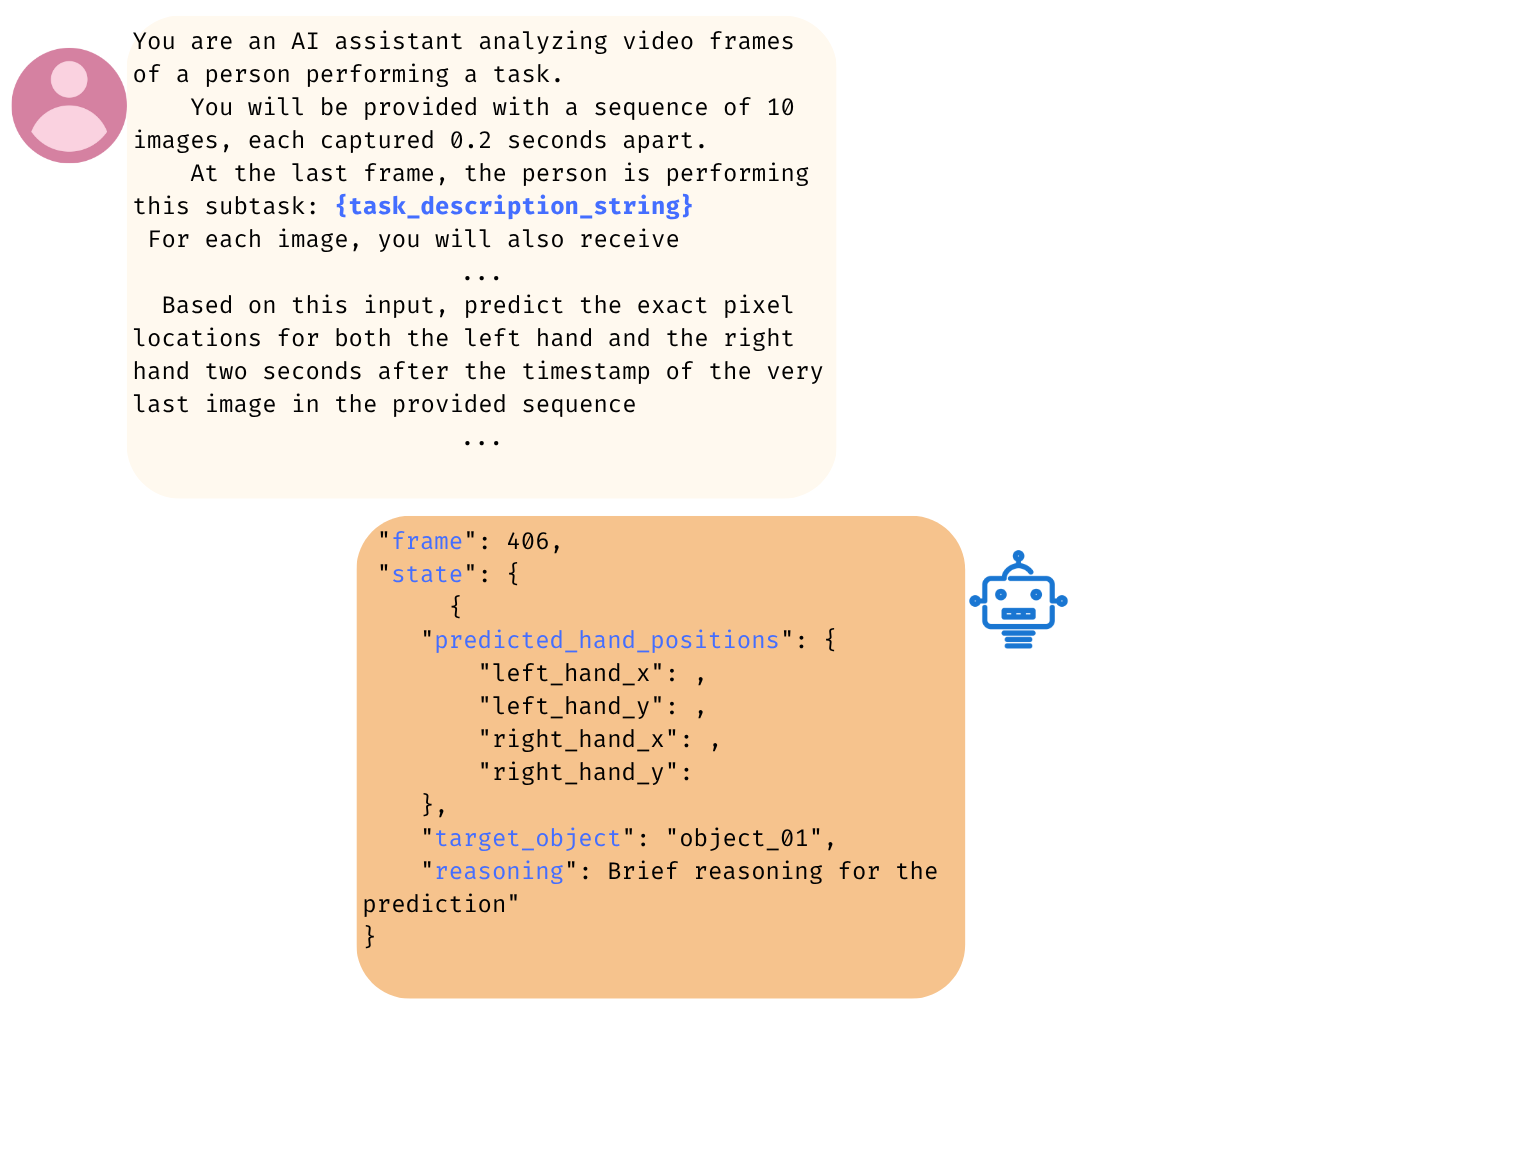
\includegraphics[width=0.48\textwidth, trim=5 0 235pt 0, clip]{s6.png}\label{fig:hand_prediction}}
    
\caption{The two-phase pipeline of the Reasoning and Intent Prediction Module: (\textbf{a}) In the first phase, the VLM uses the task graph and visual information to update the overall task state. (\textbf{b}) In the second phase, it uses this state along with a sequence of recent frames and additional context to predict the operator's future hand positions.}
    \label{fig:prediction_pipeline}
\end{figure}

\subsection{Human Motion Generation}
\label{sec:motiongeneration}
As a final, downstream step, the high-level predictions from the reasoning and intent prediction Module can drive a Motion Generation Module.
This module is crucial for visualizing the predicted intent as a full-body 3D motion. The core of this module adapts the CLoSD framework \citep{tevet2024closd}, which builds upon the Human Motion Diffusion Model (MDM) \citep{tevet2023human}. The forward diffusion process $q(x_t|x_{t-1}) = \mathcal{N}(x_t; \sqrt{\alpha_t}x_{t-1},(1-\alpha_t)I)$ gradually adds noise to a motion sequence, while the reverse process $p_\theta(x_{t-1}|x_t) = \mathcal{N}(x_{t-1}; \mu_\theta(x_t,t),\sigma_t^2 I)$ learns to denoise it by minimizing an L2 loss $\mathcal{L}_{\text{simple}} = \mathbb{E}_{x_0,t}[\|x_0 - \hat{x}_0\|_2^2]$. The model receives the previous 40 frames of motion data in HumanML3D format and synthesizes the future motion sequences for the next two seconds (60 frames). This is additionally conditioned on a textual prompt and a target joint (e.g., \texttt{right\_wrist}, \texttt{pelvis}) and its target 3D location. The Human Motion Model hence synthesizes a physically plausible and semantically guided future motion sequence. This motion sequence is subsequently visualized in a virtual representation of the real environment given by a 3D point cloud created by the perception module's depth estimation model.

\section{Framework Validation and Use Cases} \label{sec:experimental_validation}

This section validates the proposed framework by applying it to three diverse use cases. Each scenario is designed to test the framework's predictive capabilities in a different context of varying difficulty.

\subsection{Use Case 1: Chair Stacking Scenario}
This use case introduces a predictable task to demonstrate the framework's core capabilities: a person moving a toolbox from a chair and then stacking several chairs in a domestic environment, as shown in Figure \ref{fig:stack}.
\begin{figure}[H]
    \centering       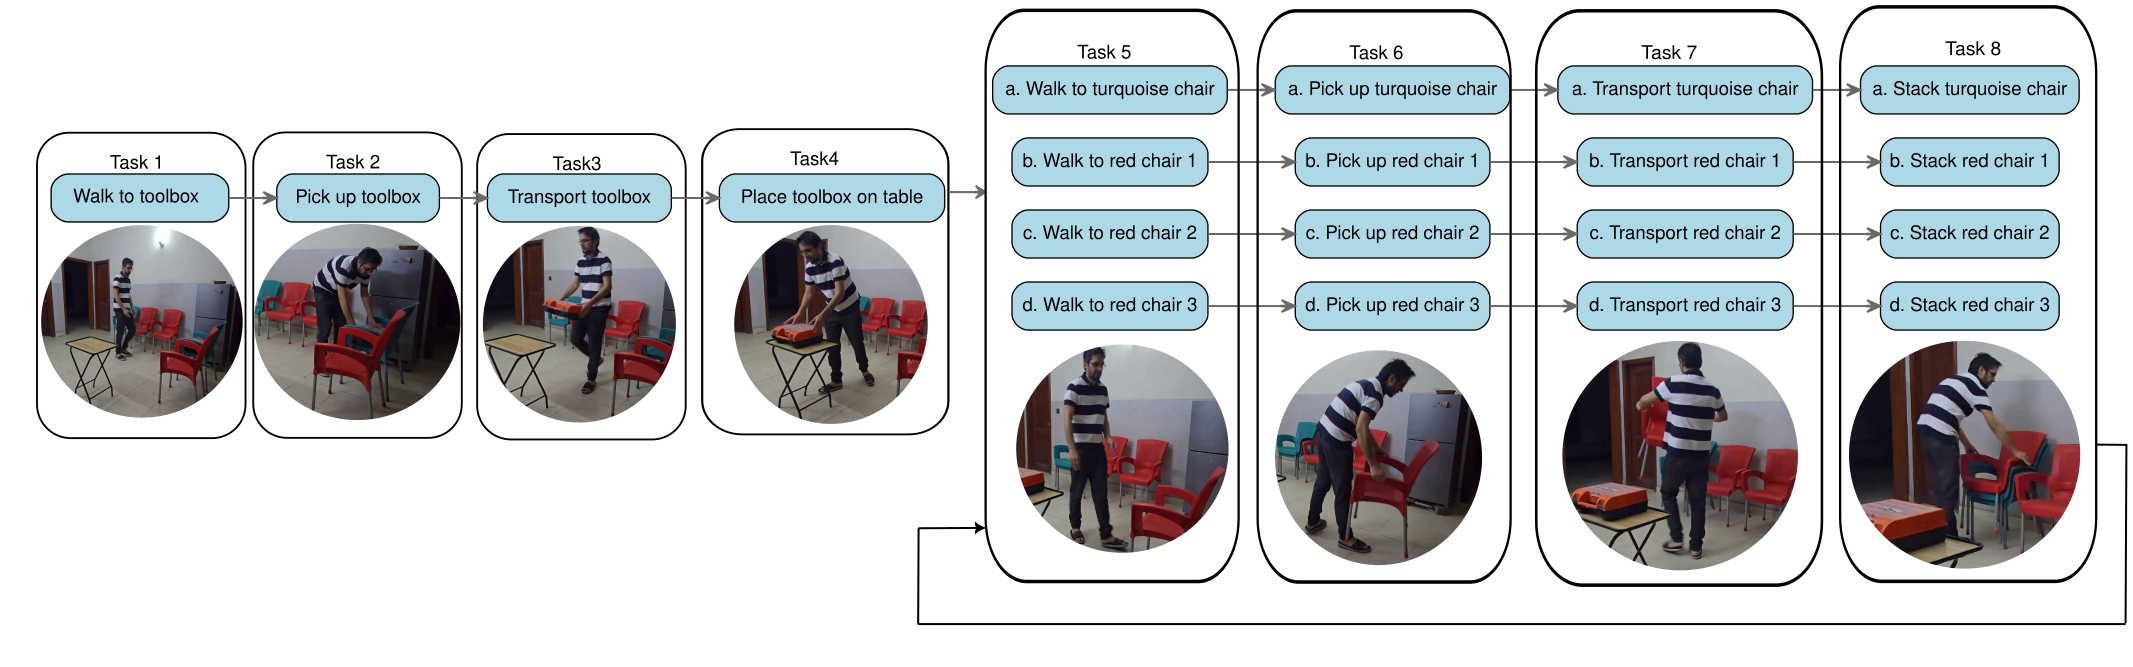
\includegraphics[width=\textwidth]{stack_task_action_graph.png} 
    \caption{Use Case: Stacking task in a domestic setting}
    \label{fig:stack}
    
\end{figure}


The initial phase involves a human-AI collaboration to define the task context.
An AI model analyzes a sample video of the task or textual instructions to propose an initial "Task Context Description."
This description includes the overall goal (e.g., "stack all chairs in the designated area"), a state representation (e.g., operator holding status, ordered list of stacked chairs), a decomposition of actions (e.g., "walk to turquoise chair", "pick up red chair",  "Transport turquoise chair"), and their dependencies.
This draft is then reviewed and refined by a human.
The LLM's output is a JSON object representing the updated state variables, including \texttt{gaze\_target}, \texttt{operator\_holding}, \texttt{num\_chairs\_stacked}, \texttt{steps\_completed}, and \texttt{steps\_available} based on the task graph.

In the first phase, the overall task state is predicted by the framework. Once the overall task state is understood, the framework can proceed to a more granular, short-term motion prediction task, as illustrated in Figure \ref{fig:stack_phase_two}. For this, the VLM is provided with a rich, multimodal context. This includes a sequence of the 10 most recent image frames, captured at intervals of 0.2 seconds. Each frame is augmented with vital information: a heatmap indicating the operator's gaze target, an overlay of the estimated human pose, and the precise, normalized pixel coordinates and velocities of the operator's hands. The model is also given the current sub-task description textually (e.g., "Transport turquoise chair"). The VLM's objective is to analyze this temporal sequence and, informed by the task context, predict the exact pixel locations of the left and right hands two seconds after the final frame in the sequence. This approach moves beyond simple kinematic extrapolation, compelling the model to make a physically and semantically plausible forecast based on an understanding of the human's immediate goal.

\begin{figure}[H]
    \centering       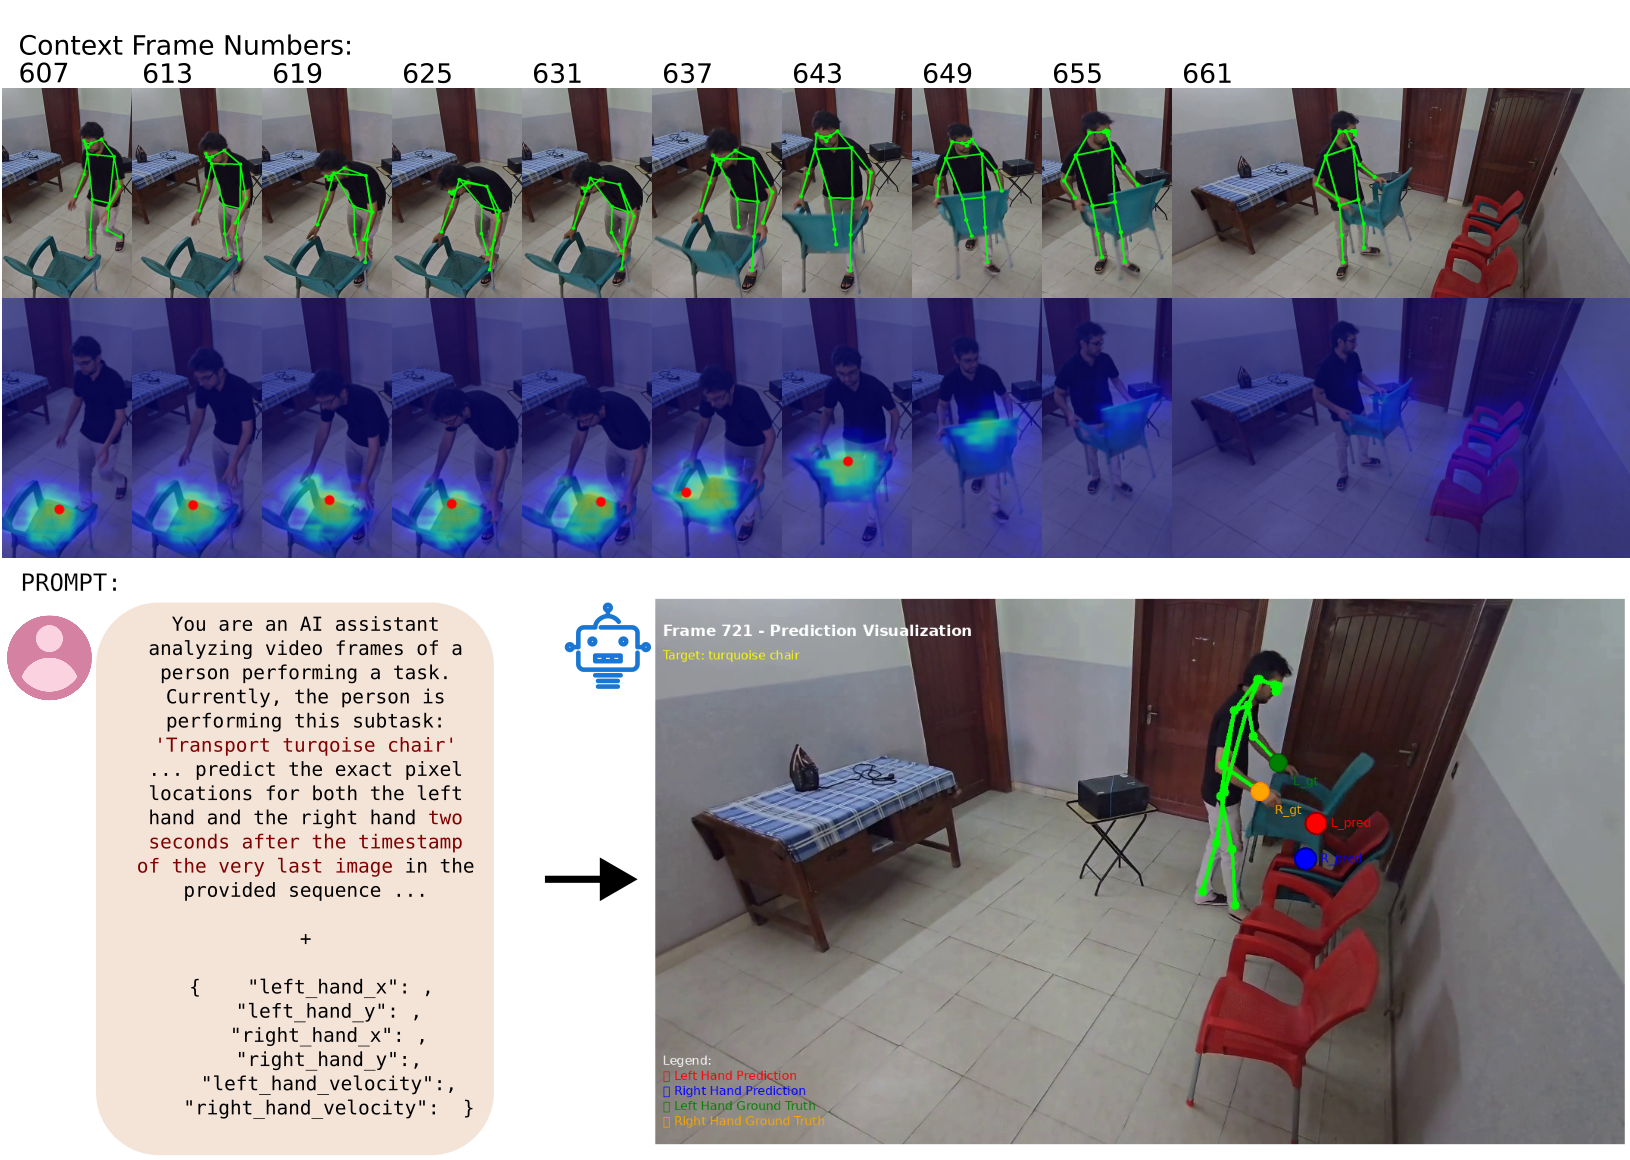
\includegraphics[width=\textwidth]{Stack_phase_two.png} 
    \caption{Hand position prediction for Stacking Scenario}
    \label{fig:stack_phase_two}    
\end{figure}


Depending on the approach, the x,y pixel coordinates or the target object can be processed to find the world-frame coordinates of the target joint, as described in Section \ref{sec:sceneunderstanding}. This is further employed in the motion generation module. Figure \ref{fig:stacking_prediction} illustrates the motion generation results for the chair-stacking use case while performing Task 4: 'Place toolbox on chair'.

\begin{figure}[H]
\begin{adjustwidth}{-\extralength}{0cm}
    \centering
    \subfloat[][]{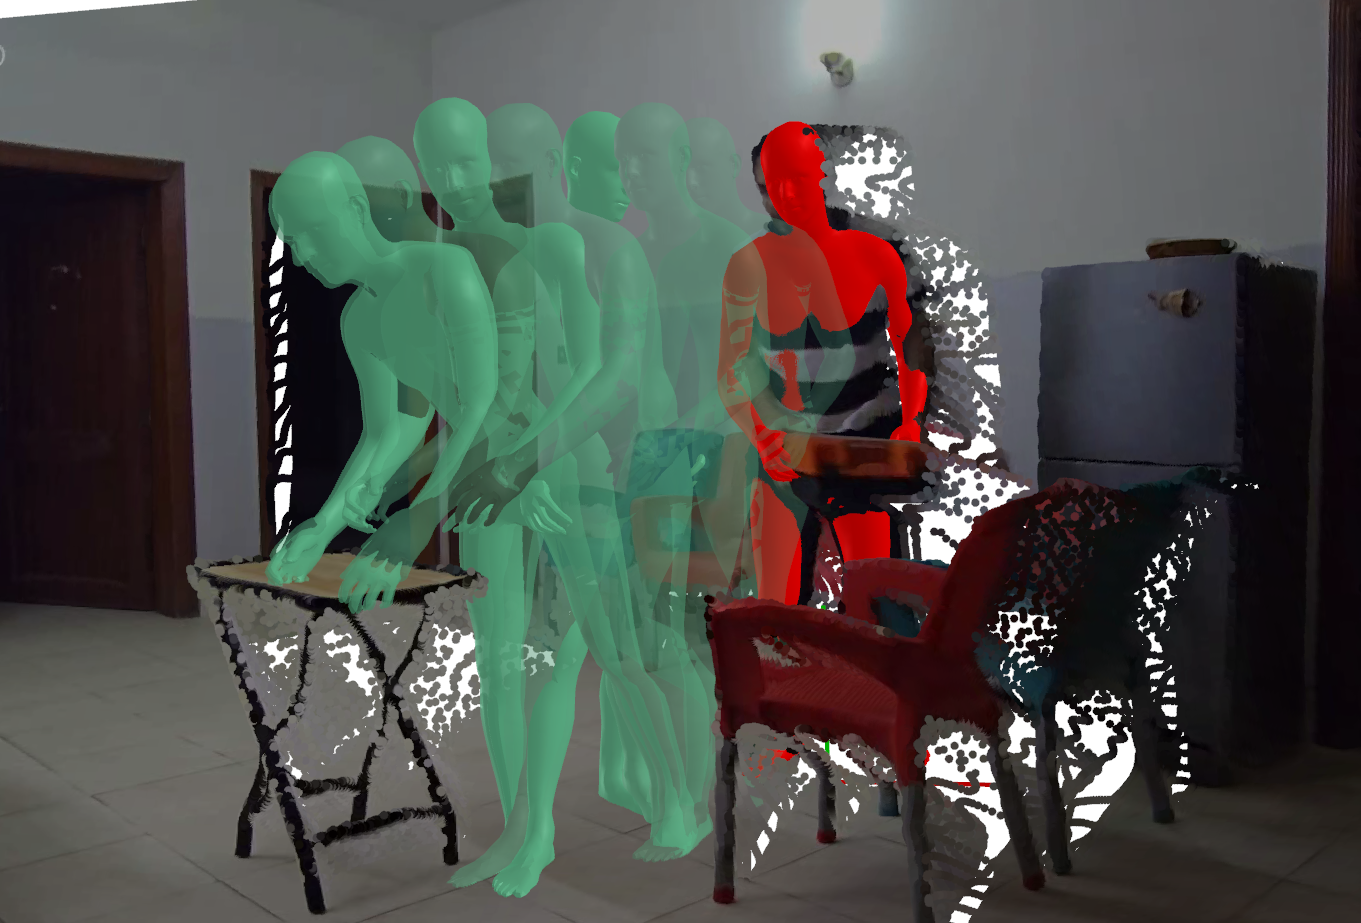
\includegraphics[width=0.6\textwidth,  trim=0 0 0 40, clip]{s3.png}}          
    \subfloat[][]{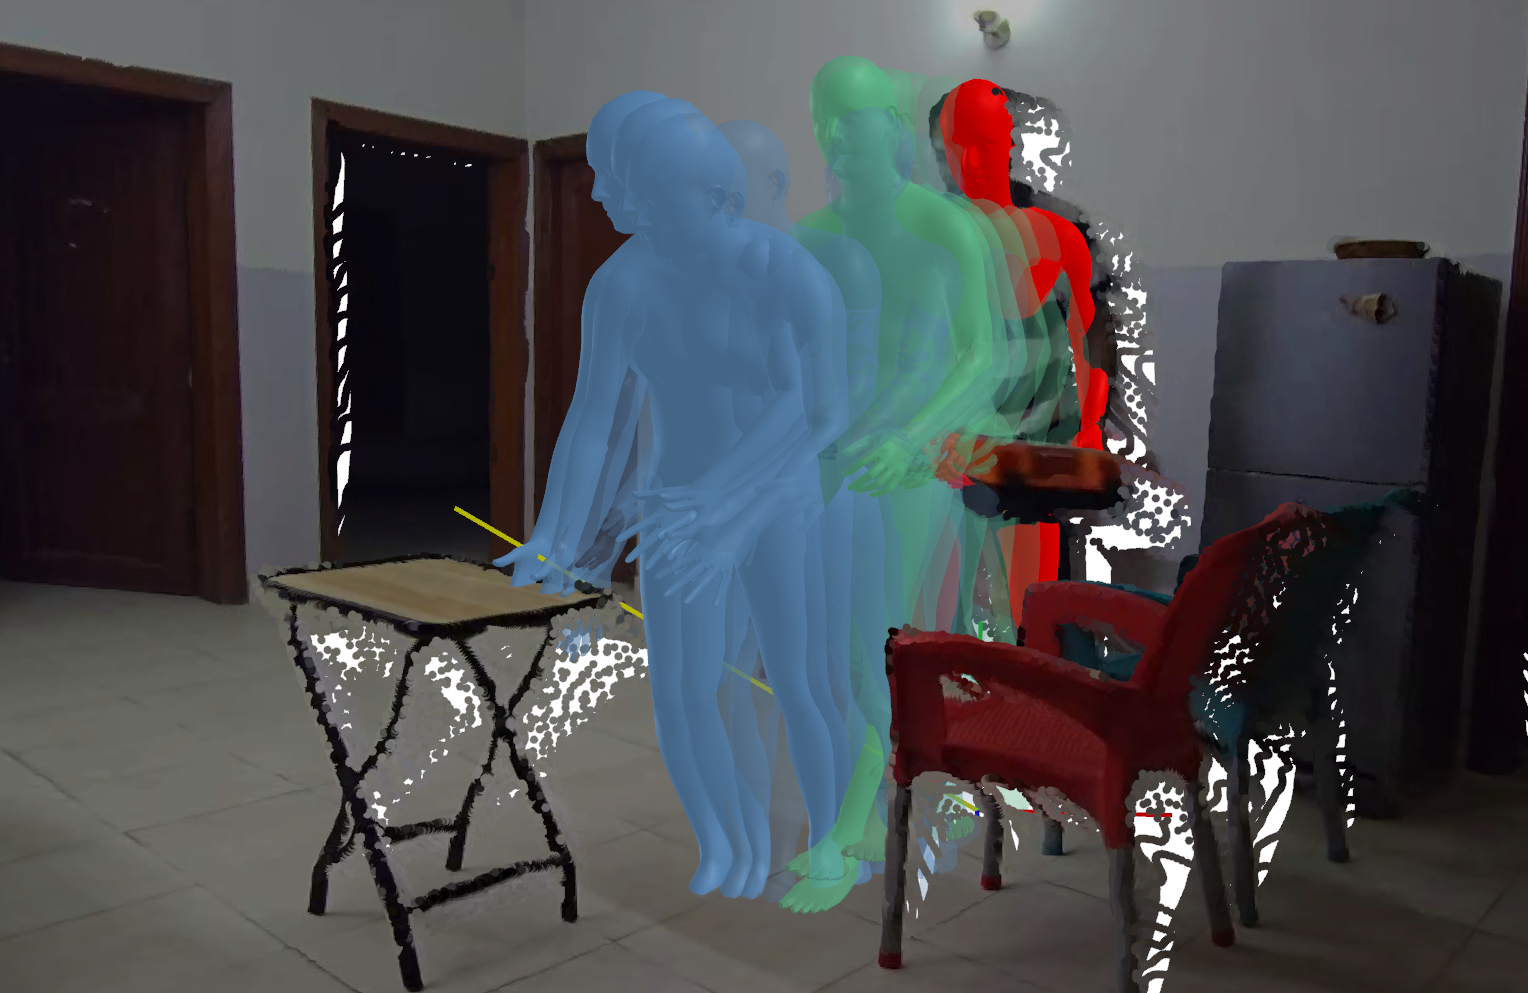
\includegraphics[width=0.6\textwidth, trim=0 0 0 0, clip]{s4.png}}
\end{adjustwidth}
    \caption{Visualizations for Task 4 within the Stacking Use-case (\textbf{a}) Starting position in red and Ground truth of the human's motion, shown in green as they put the toolbox on the table. (\textbf{b}) Generated motion, shown in blue, with the yellow line representing target vector for the position of the left wrist}
    \label{fig:stacking_prediction}
\end{figure}

\begin{figure}[H]
\centering
\subfloat[\centering]{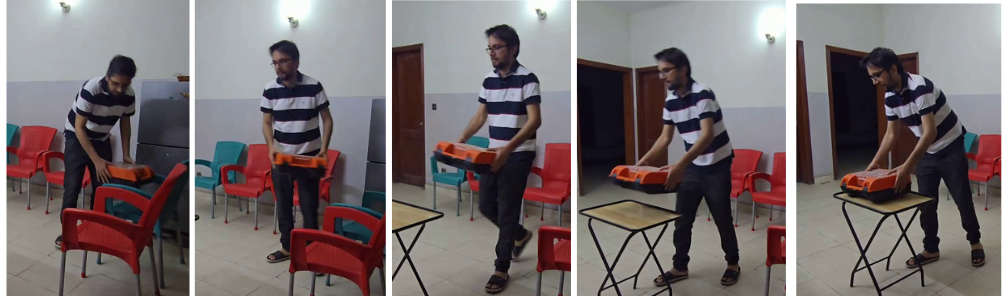
\includegraphics[width=\linewidth]{4cr.png}}

\vfill
\subfloat[\centering]{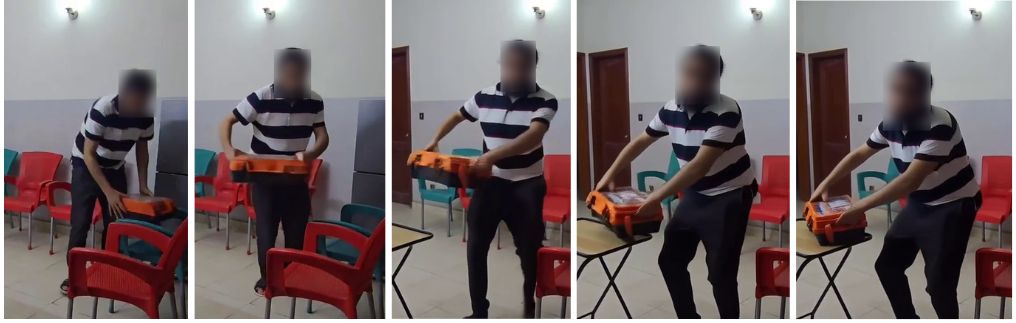
\includegraphics[width=\linewidth]{5cr.png}} 

\caption{Comparison of actual 
and AI-generated motion frames for placing a toolbox. (\textbf{a}) Actual motion frames. (\textbf{b}) AI-Generated motion frames}
\label{fig:actual_vs_generated}
\end{figure}

The modularity of the framework allows for flexible integration of alternative motion visualization methods. One such alternative is the use of AI driven image-to-video generation tools. In this approach, the reasoning and intent prediction module of the framework generates a text prompt describing the predicted intent. The prompt and the starting frame of the sequence are passed to a video generation model. This method is not suitable for real-time prediction due to significant computational latency. Additionally, it can sometimes lead to physically implausible hallucinations. However, it serves as a powerful tool for visualization. Figure \ref{fig:actual_vs_generated} illustrates a comparison between actual motion frames and those synthesized by the Wan2.1 framework \citep{wan2025} using this technique.


\subsection{Use Case 2: Assembly Task}
The second use case leverages the Human Assembly Video Dataset (HaVID) \citep{havid} to evaluate the framework's performance on fine-grained industrial assembly tasks.
HaVID's detailed annotations of actions provide a rich ground truth for assessing intent prediction.
This use case demonstrates the framework's applicability to tasks with clear SOPs, common in manufacturing environments \citep{David2023}. PDF assembly instructions and exploded assembly drawings for a task like HaVID's "Cylinder Assembly" are first used,  with AI assistance, to generate a comprehensive action graph (DAG) and a suitable state representation (Figure \ref{fig:havid_dag}). Given the potential for variations in assembly sequences, multiple valid paths through the DAG are considered.
\begin{figure}[H]
    \centering
        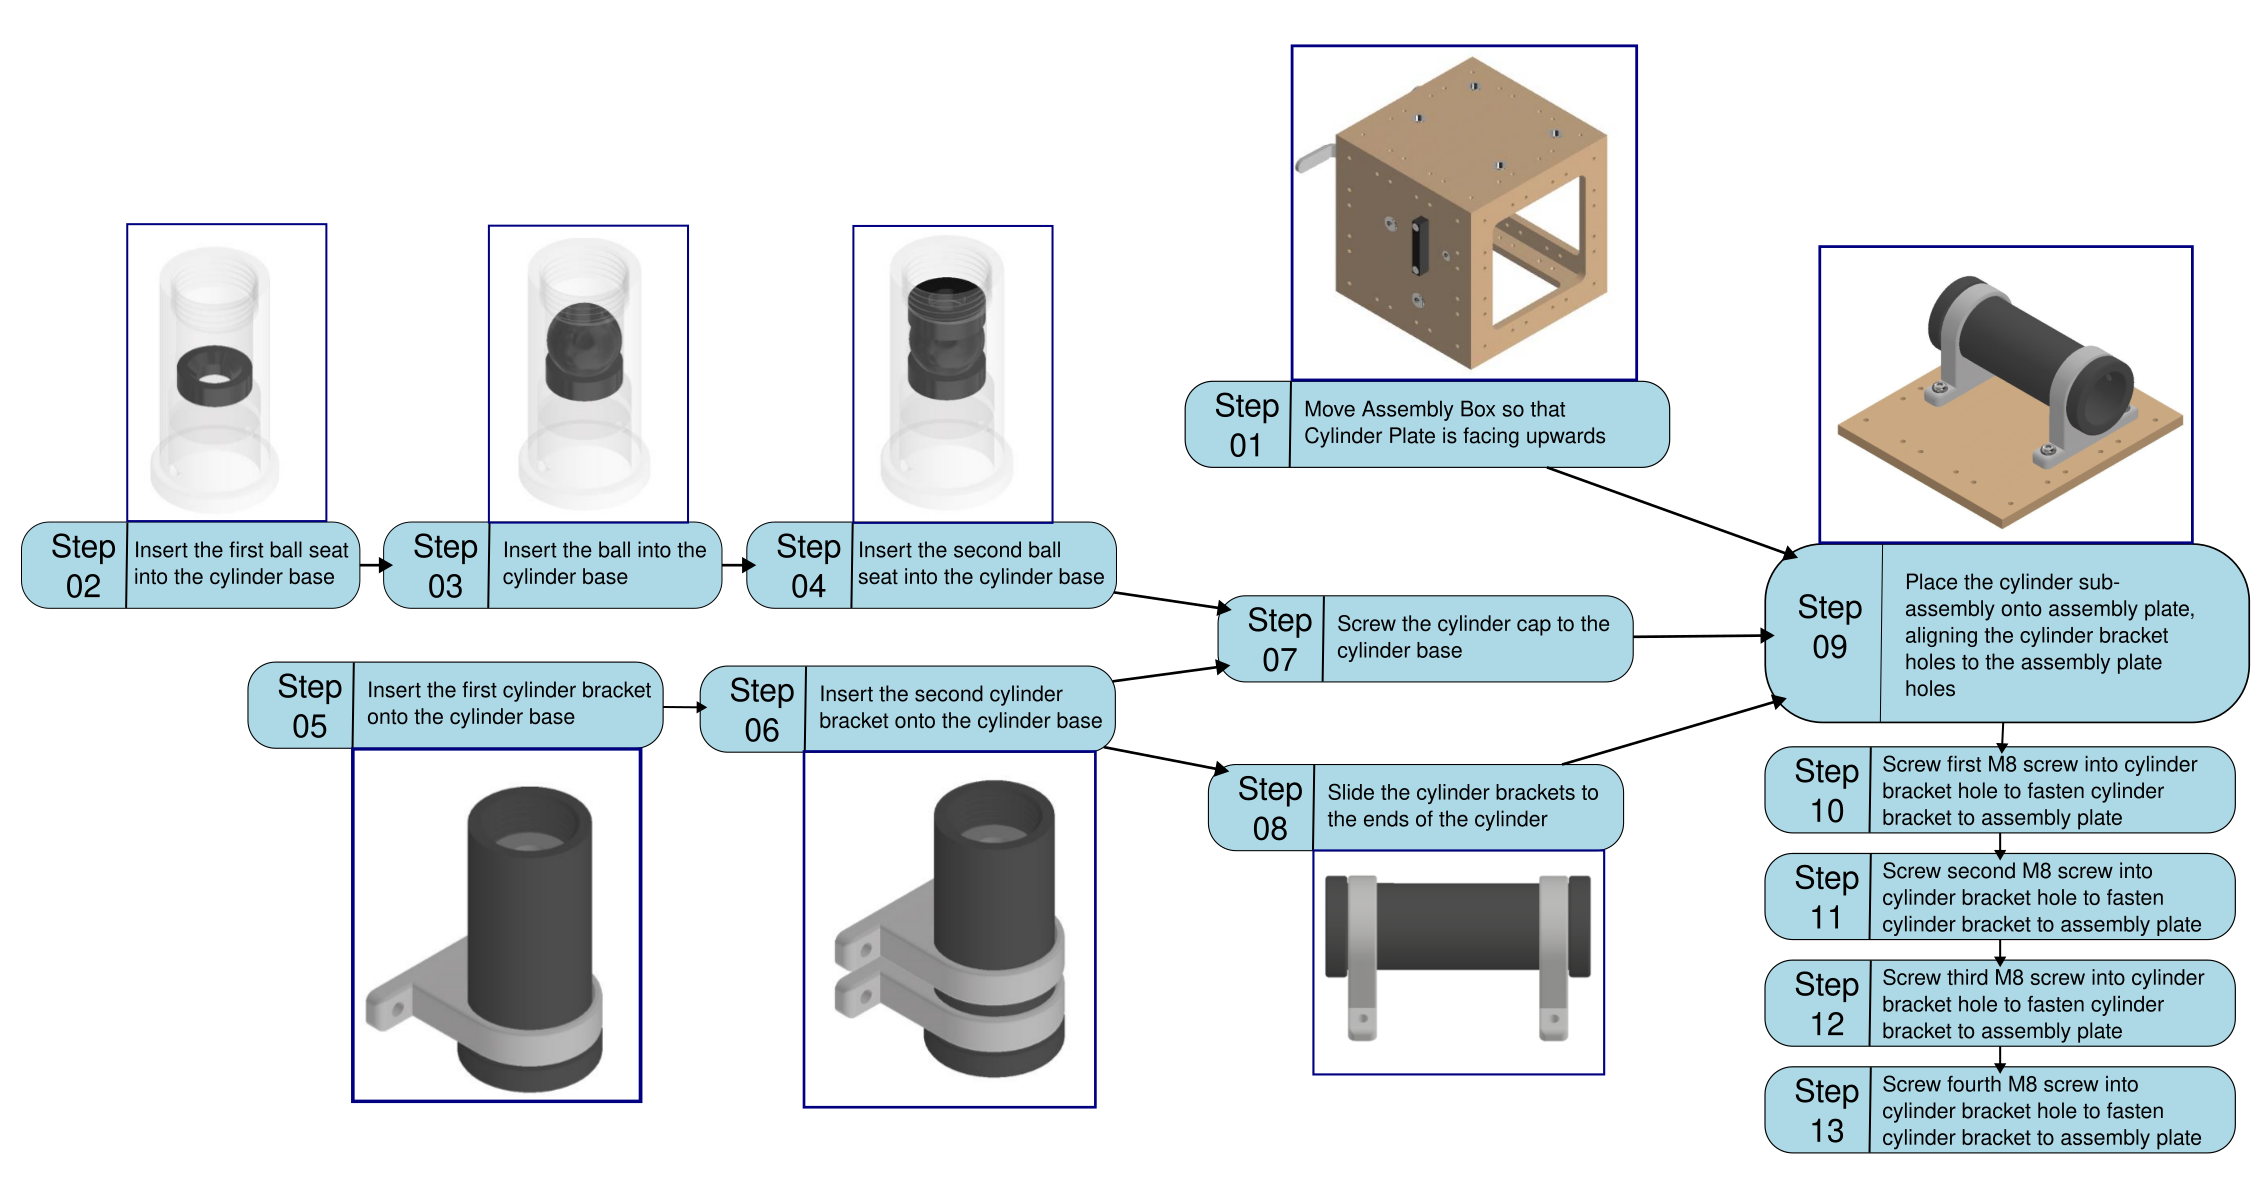
\includegraphics[width=\textwidth]{havid_task_graph.png} 
        \caption{Directed Action Graph for Assembly Task based on the HAViD dataset.}
        \label{fig:havid_dag}
\end{figure}
Ground-truth states for selected HaVID video segments are then generated by translating HaVID's temporal annotations into the state representation format used, a process facilitated by AI with human oversight.
These ground-truth states serve both for in-context learning examples and for evaluation.
As detailed in the previous use-case, the system first predicts the system state.  This is followed by a fine-grained prediction of hand positions to forecast the operator's immediate movements, applying the same multimodal analysis approach (Figure \ref{fig:havid_phase_two}). 

\begin{figure}[H]
    \centering       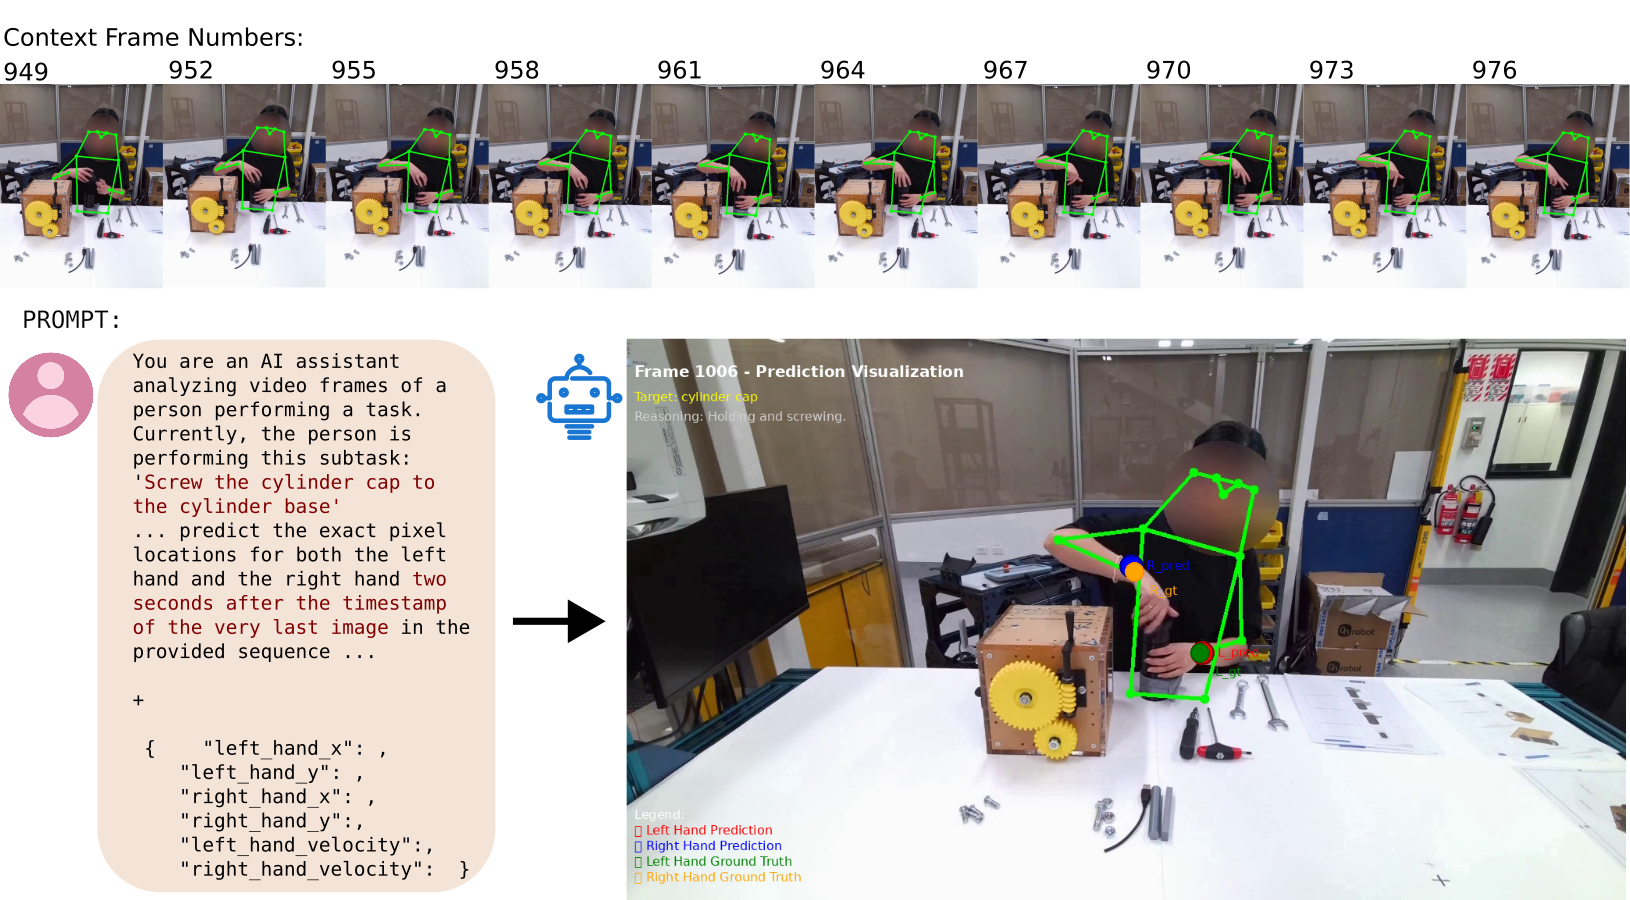
\includegraphics[width=\textwidth]{havid_phase_two.png} 
    \caption{Hand position prediction for Assembly Scenario}
    \label{fig:havid_phase_two}    
\end{figure}

The results of this intent-aware forecasting are then used to generate plausible future motion, as visualized in Figure \ref{fig:havid_motion_prediction}.

\begin{figure}[H]
\begin{adjustwidth}{-\extralength}{0cm}
    \centering
    \subfloat[][]{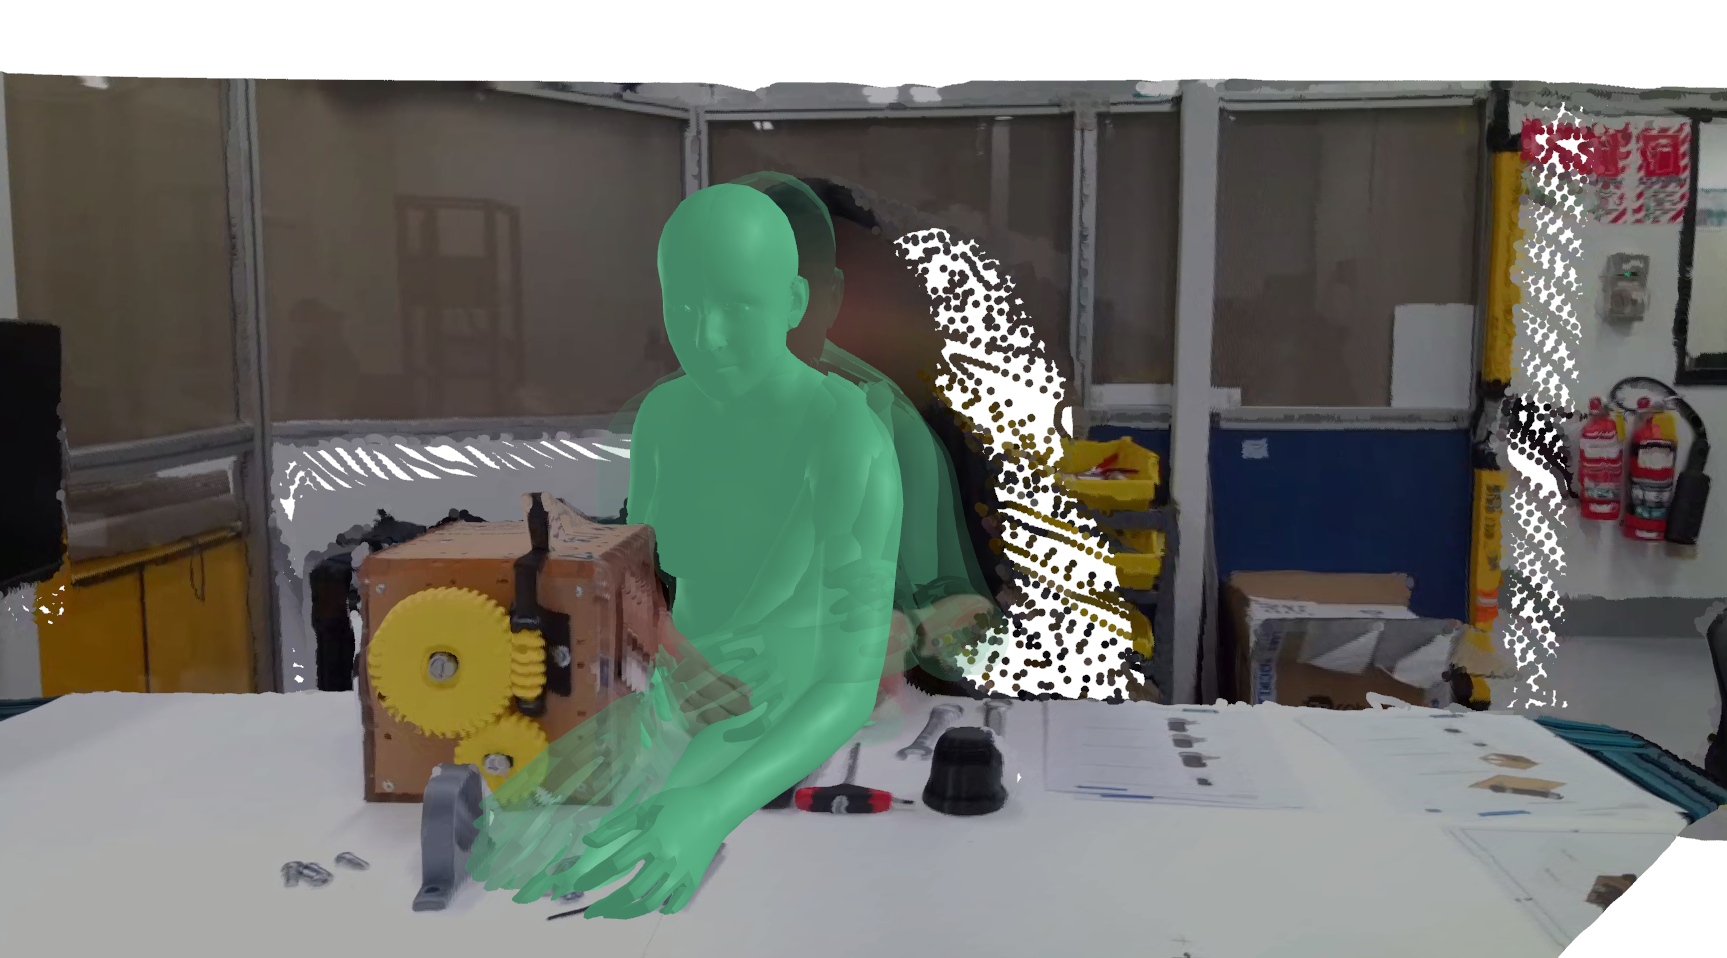
\includegraphics[width=0.6\textwidth, trim=10 0 360 25, clip]{s2.png}}
    \subfloat[][]{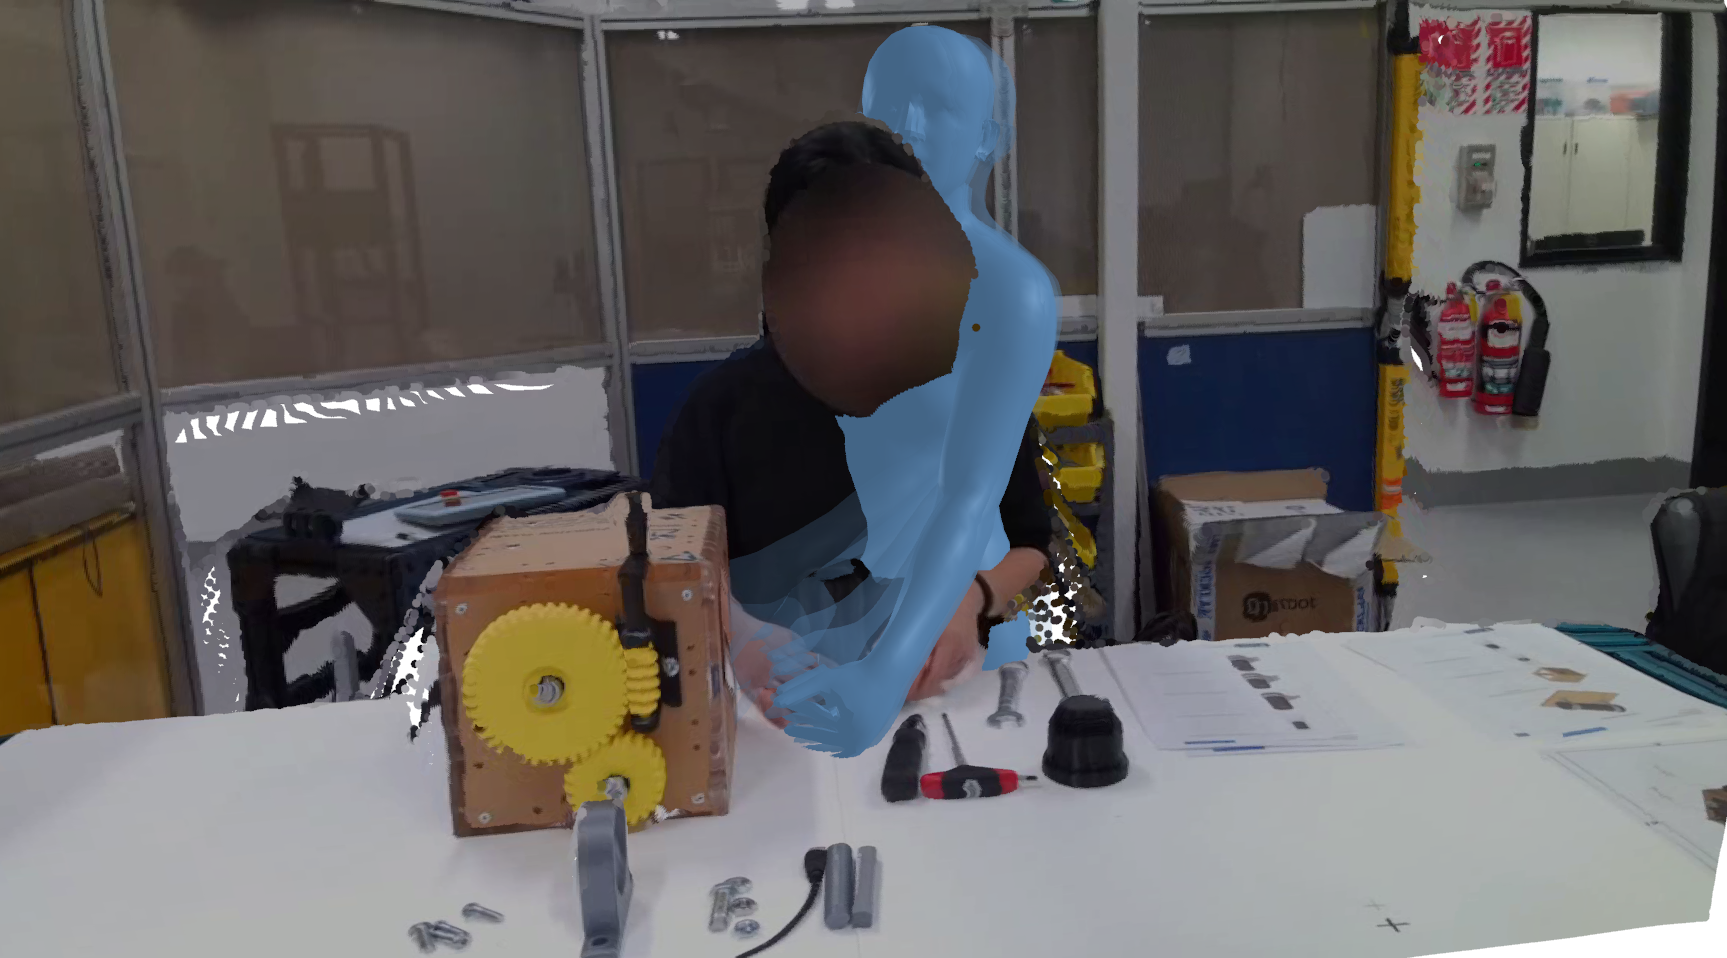
\includegraphics[width=0.6\textwidth, trim=0 0 280 25, clip]{s1.png}}
\end{adjustwidth}
    \caption{Visualizations within the HAVID Assembly use case. (\textbf{a}) Ground truth of the human's motion over the previous 1 second, shown in green. (\textbf{b}) Generated motion, shown in blue, indicating the expected motion of the human's hand.}
    \label{fig:havid_motion_prediction}
\end{figure}

\subsection{Use Case 3:  Cooking Scenario}
To test the framework against long-horizon and complex tasks, the third use case utilizes the EgoExo4D dataset \citep{egoexo}. This dataset is particularly suitable for this research, as it includes synchronized egocentric and exocentric video streams, along with rich temporal annotations, including task and keystep-level labels. A challenging noodle cooking scenario was selected, for which multiple recordings from the same kitchen location are available, providing ideal in-context learning examples.

\begin{figure}[H]
    \centering       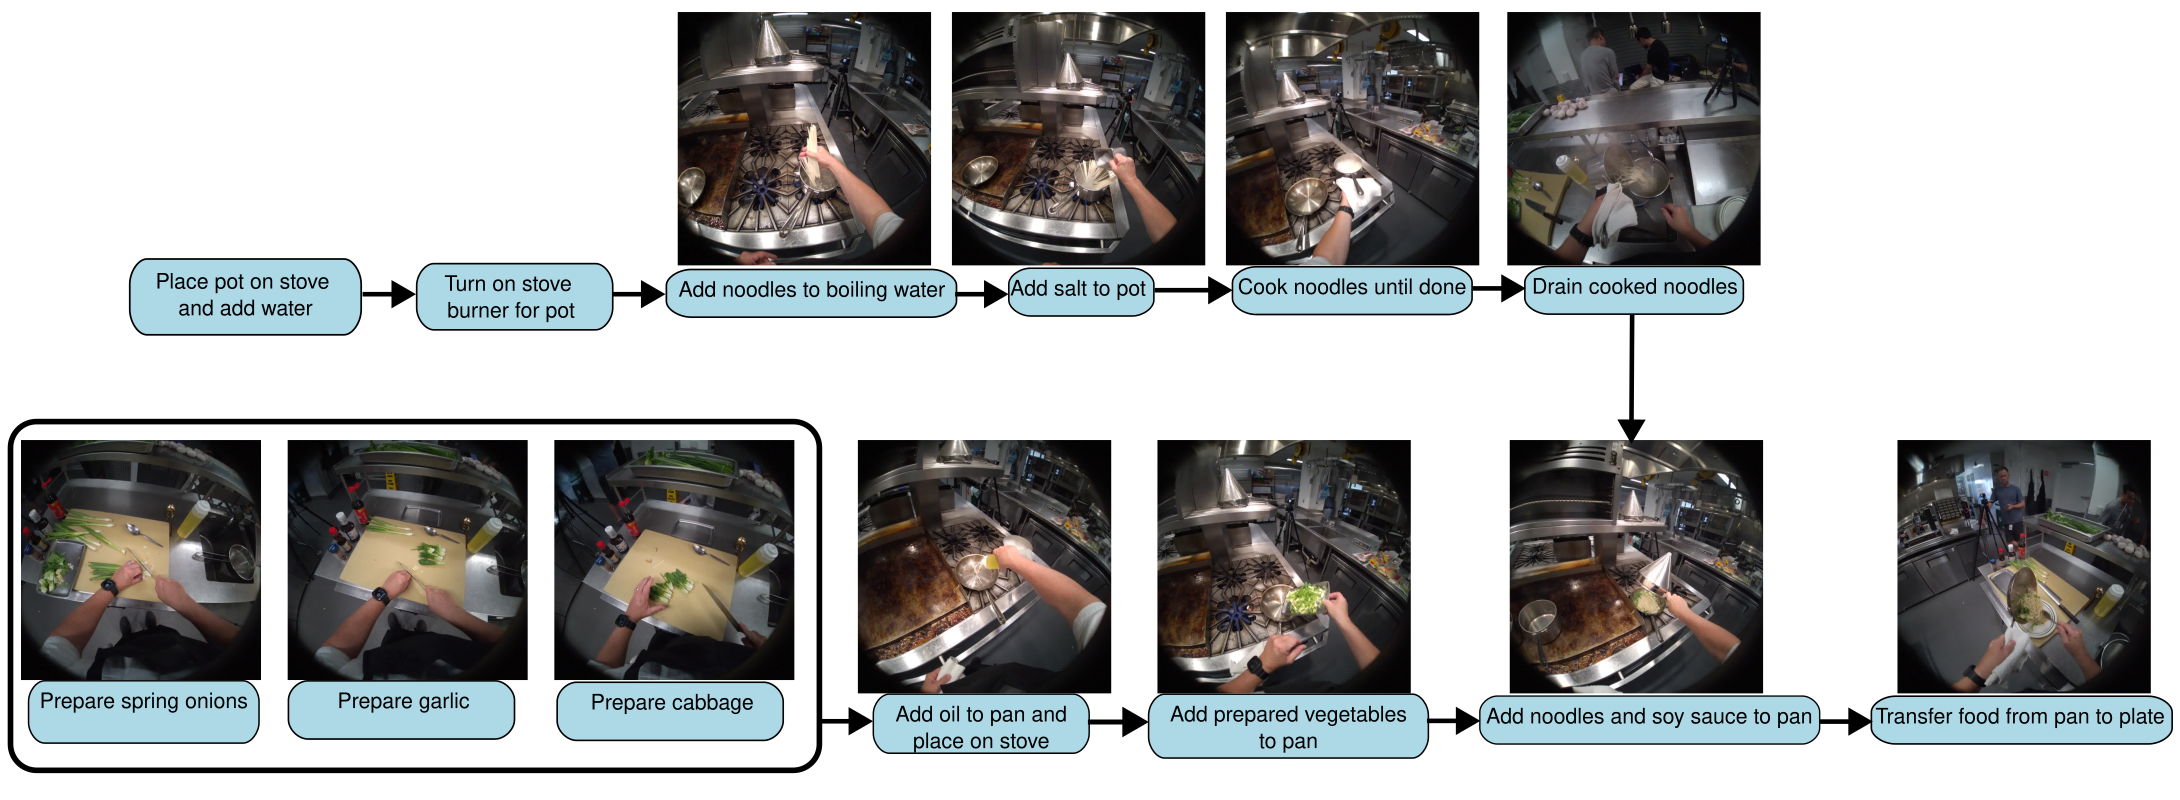
\includegraphics[width=\textwidth]{cooking_task_graph.png} 
    \caption{Sample action graph for Cooking Scenario}
    \label{fig:cooking_dag}    
\end{figure}

The cooking task (Figure \ref{fig:cooking_dag})  introduces distinct challenges not as prevalent in the other scenarios. It involves a much larger time horizon, and the state of the task is often ambiguous and not easily discernible from visual cues alone. For instance, by observing a single frame or even a short sequence of an idle cook, it is difficult to determine if the vegetables are fully chopped or if the noodles have finished boiling. Furthermore, the scenario includes significant periods of inactivity or "waiting" where the operator's next action is not imminent. While the overall task has a clear structure, the cook does not need to move from completing one sub-task to immediately carrying out the next, making the precise timing of future actions inherently unpredictable.

Despite these complexities, the framework follows the established two-phase prediction process: the AI agent first predicts the current action or task state, which is then used to inform a fine-grained hand position prediction. A key distinction in this use case is the augmentation of the VLM's context with first-person egocentric frames, which are provided to the model along with the primary exocentric view and gaze data, as shown in Figure \ref{fig:cooking_phase_two}. Note that only half the context frames are shown in the Figure for brevity. The RGB frames provided as context are also omitted.

\begin{figure}[H]
    \centering       
    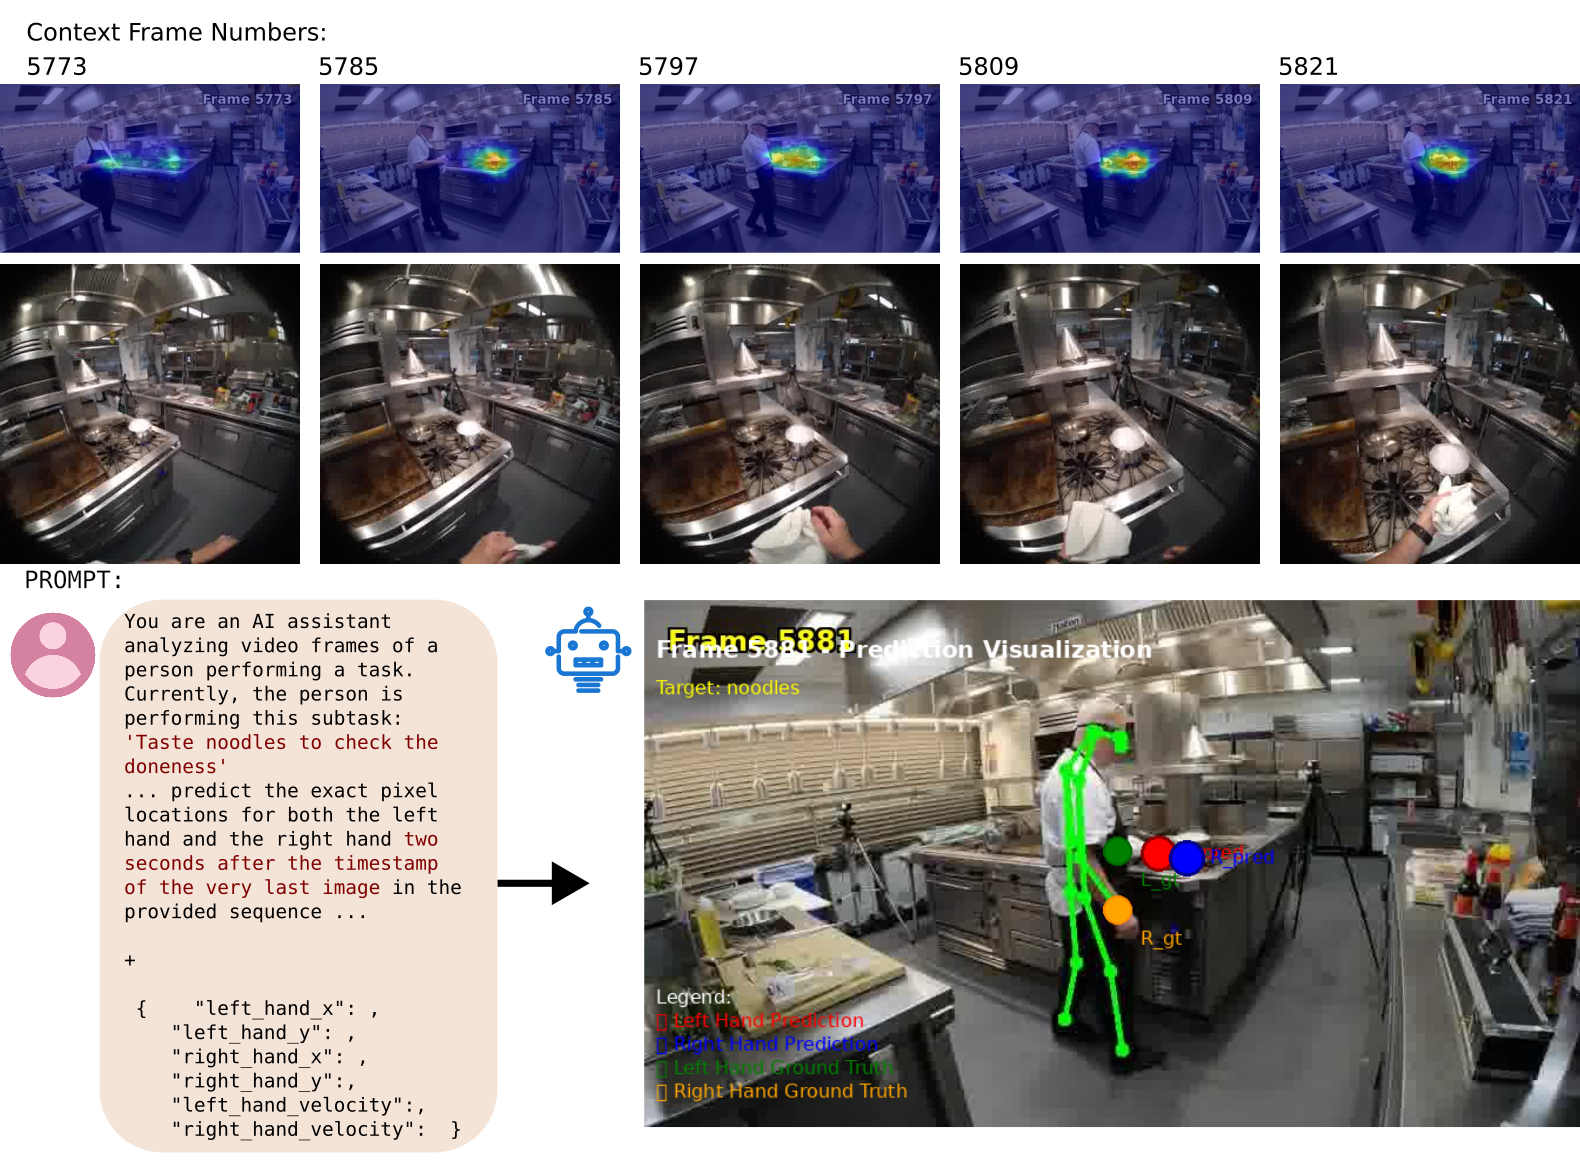
\includegraphics[width=\textwidth]{Cooking_phase_two.png}
    \caption{Hand position prediction for Cooking Scenario.}
    \label{fig:cooking_phase_two}    
\end{figure}

\section{Framework Performance Evaluation}
\label{sec:eval}
Evaluating the performance of the proposed framework requires a multi-faceted approach, as no single, established benchmark currently exists for the end-to-end task of context-aware human intention and motion prediction. Our work aims to lay the groundwork for such a benchmark. We therefore define a set of specialized metrics to assess both the high-level semantic understanding (Phase 1) and low-level motion prediction accuracy (Phase 2), and report results across diverse use cases.

To evaluate the frame-wise prediction of the task state, we use a weighted F1 score, which is well-suited for this multi-label classification problem  \citep{F1ref}.

\begin{linenomath}
\begin{equation}
    F1 = 2 \cdot \frac{P \cdot R}{P + R} = \frac{2TP}{2TP + FP + FN}
\end{equation}
\end{linenomath}

where TP, FP, and FN are the counts of true positives, false positives, and false negatives, respectively, and P and R are precision and recall, respectively. The overall Task State Accuracy (TSA) is calculated as a weighted sum of the F1-scores for the classification of completed, in-progress, available steps, and the immediate next step:

\begin{linenomath}
\begin{equation}
\text{TSA Score} = (w_c F1_c + w_p F1_p + w_a F1_a+w_nF1_n) 
\end{equation}
\end{linenomath}

where $F1_c, F1_p, F1_a, F1_n$ are the F1-scores for the completed, in-progress, available steps, and immediate next steps respectively, with weights $w_c, w_p, w_a$, and $w_n$ 

Table \ref{tab:phase_one_results} presents performance figures for the Task State Accuracy. A central observation is the trade-off between accuracy, latency, and cost. A baseline strategy of providing only a single image to the Vision-Language Model (VLM) consistently underperforms due to the lack of historical context or "memory". For a balance of performance and latency, a rolling context window (RCW) strategy was employed, using 10 frames spaced one second apart, augmented with the predicted state from the initial frame. However, this approach is prone to consistency bias; if the model erroneously determines a step to be completed, it often fails to revise this belief, causing subsequent predictions to suffer. When this strategy is tested with the ground-truth state provided as context, performance is significantly higher and becomes less dependent on model size, with smaller models also performing well. This approach, using the low-latency Gemini 2.5 Flash-Lite model, can achieve near real-time predictions within 2-3 seconds, whereas Gemma and the standard Gemini 2.5 Flash models average closer to 10 seconds.
The best accuracy is achieved using in-context learning, where a full, similar example video and its corresponding ground-truth state evolution are provided in the prompt. While effective, the associated latency makes this approach impractical for real-time applications with current technology. 

The inclusion of additional visual cues yielded mixed results. A significant improvement was observed by incorporating egocentric first-person views in the EgoExo4D-based Cooking scenario, where performance increased from 0.568 to 0.629, a 10.7\% improvement.  In contrast, adding gaze target heatmaps, when averaged over all experiments, led to only an inconsistent and marginal performance 3\% increase from 0.667 to 0.688. We theorize that the egocentric perspective provides a more reliable signal of operator attention than gaze target heatmaps. Also, this suggests that while gaze data is valuable, its primary utility may be in predicting short-term hand motion, as discussed later, rather than for long-horizon task state analysis.

\begin{table}[h!]
% Use resizebox to force the table to fit within the text width
\resizebox{\textwidth}{!}{%
\begin{tabular}{llcccccc}
\toprule
& & \multicolumn{3}{c}{\textbf{Task-Specific Score}} & \multicolumn{2}{c}{\textbf{Performance}} \\
\cmidrule(lr){3-5} \cmidrule(lr){6-7}
\textbf{Exp. Group} & \textbf{Model} & \textbf{Stack} & \textbf{Assembly} & \textbf{Cooking} & \textbf{Overall} & \textbf{Rank} \\
\midrule
Single Image & Gemini 2.5 Flash Lite & 0.557 & 0.367 & 0.285 & 0.403 &  \\
\midrule
\multirow{4}{*}{RCW with Ground Truth} & Gemini 2.5 Pro & 0.784 & 0.794 & 0.726 & 0.768 & 1 \\
& Gemini 2.5 Flash & 0.763 & 0.781 & 0.721 & 0.755 & 2 \\
& Gemini 2.5 Flash Lite & 0.703 & 0.724 & 0.813 & 0.747 & 3 \\
& Gemma-27B & 0.674 & 0.776 & 0.689 & 0.713 & 4 \\
\midrule

\multirow{3}{*}{In-Context Learning} & Gemini 2.5 Flash & 0.793 & 0.634 & 0.703 & 0.710 & 1 \\
& Gemini 2.5 Pro & 0.850 & 0.689 & 0.578 & 0.706 & 2 \\
& Gemini 2.5 Flash Lite & 0.703 & 0.637 & 0.571 & 0.637 & 3 \\
\midrule

\multirow{4}{*}{RCW with Predicted State} & Gemini 2.5 Pro & 0.780 & 0.753 & 0.520 & 0.684 & 1 \\
& Gemini 2.5 Flash & 0.735 & 0.679 & 0.535 & 0.650 & 2 \\
& Gemini 2.5 Flash Lite & 0.695 & 0.642 & 0.567 & 0.635 & 3 \\
& Gemma-27B & 0.634 & 0.659 & 0.478 & 0.590 & 4 \\
 
\bottomrule
\end{tabular}
}
\caption{Aggregated performance scores and rankings for Task State Accuracy}
\label{tab:phase_one_results}
\end{table}

An effective strategy for large language models should achieve high performance with minimal computational cost. Figure~\ref{fig:performance_vs_tokens} illustrates the trade-off between performance and the average number of tokens generated, a proxy for computational expense.

While providing more context can enrich a model's understanding, this approach is not without drawbacks. Beyond the obvious increases in latency and cost, simply allocating more test-time compute by expanding the context can be actively detrimental to performance. Recent work has highlighted the phenomenon of inverse scaling in test-time compute, where models paradoxically perform worse as they are given more computational resources to generate a response \citep{inversescaling}. This suggests that models can overthink or get lost in an unnecessarily large context, leading to performance degradation. The ICL strategy, with its massive token count, runs a higher risk of encountering this issue. The RCW methods, by being more selective with the provided context, not only reduce latency and costs but also mitigate the risk of this inverse scaling, demonstrating a more robust and efficient approach.

\begin{figure}[H]
    \centering
    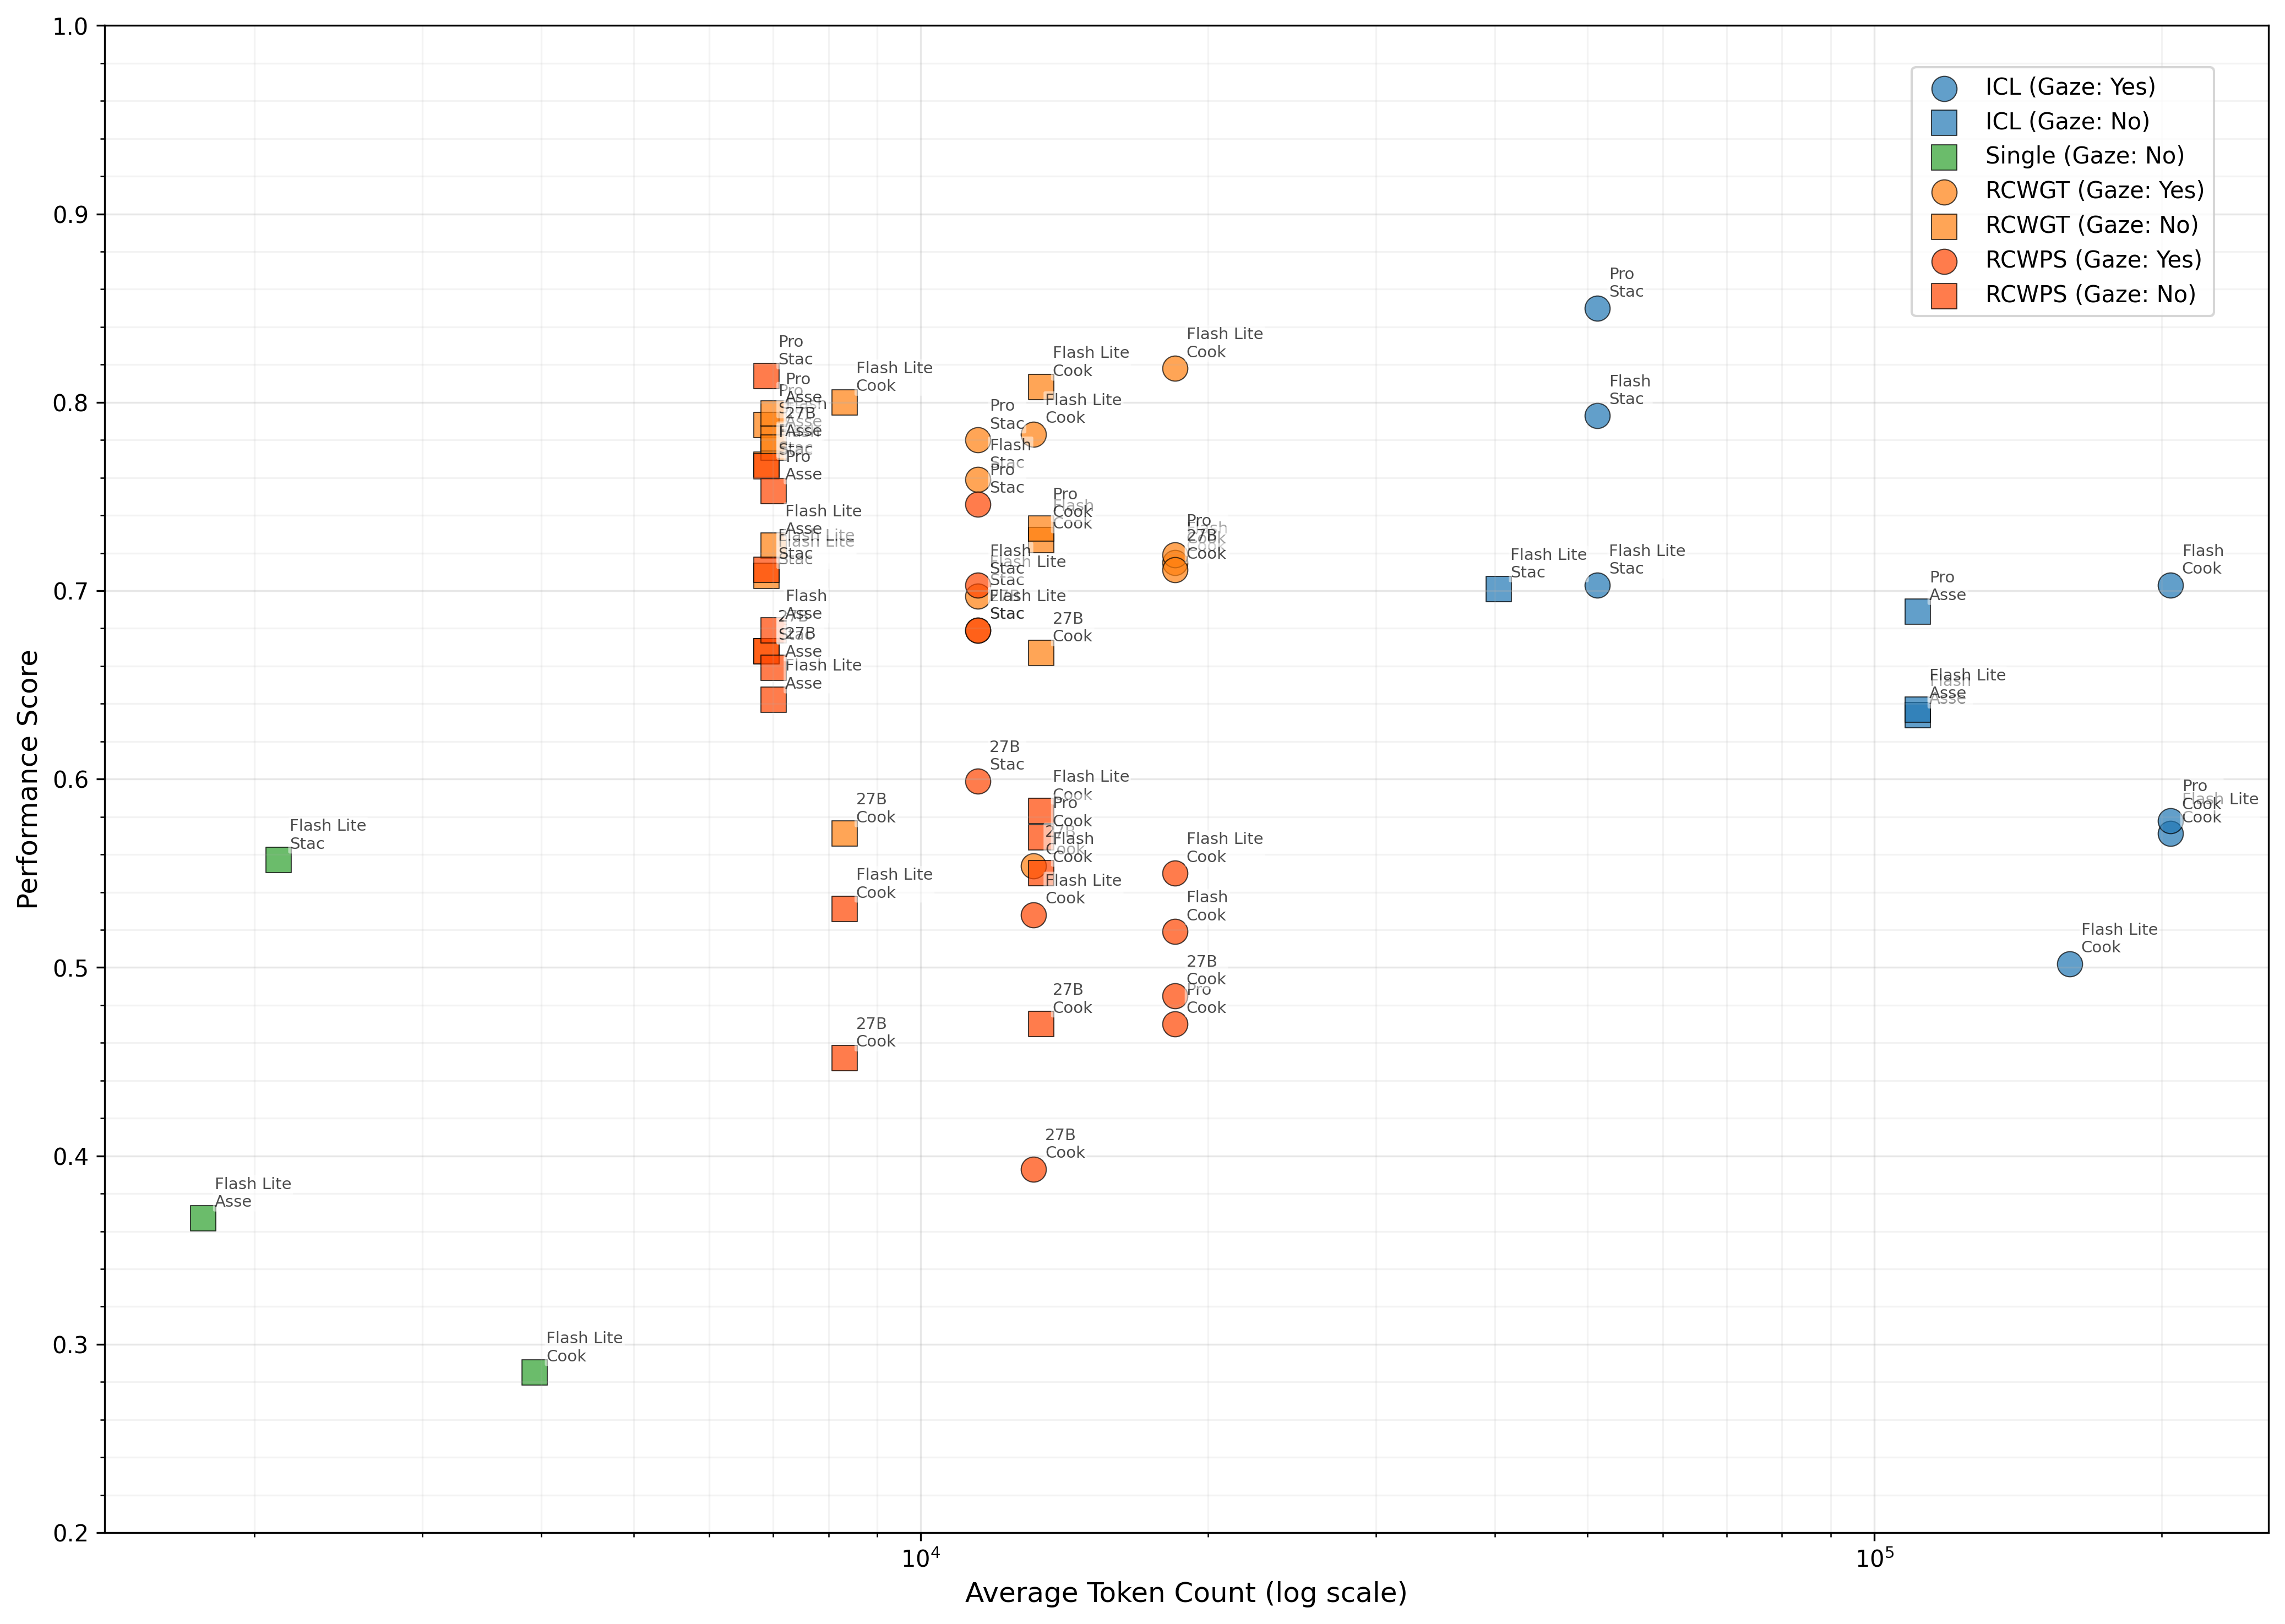
\includegraphics[width=\textwidth]{token_performance_combined.png}
    \caption{Performance score versus the average number of tokens per generation}
    \label{fig:performance_vs_tokens}
\end{figure}

The temporal aspect of predictions is critical. The timeliness of the determination that a step is completed was plotted for each use case. The results show good agreement for the Stacking and HaVID scenarios. However, the prediction of subtask completion times for the Cooking scenario is less accurate, which is attributed to the ambiguous nature and prolonged waiting periods inherent to that task. The visualization for the best-performing models for each use case is shown in Figure \ref{fig:timing_analysis}

\begin{figure}[H]
\begin{adjustwidth}{-\extralength}{0cm}
    \centering
    \subfloat[][Use Case: Stacking]{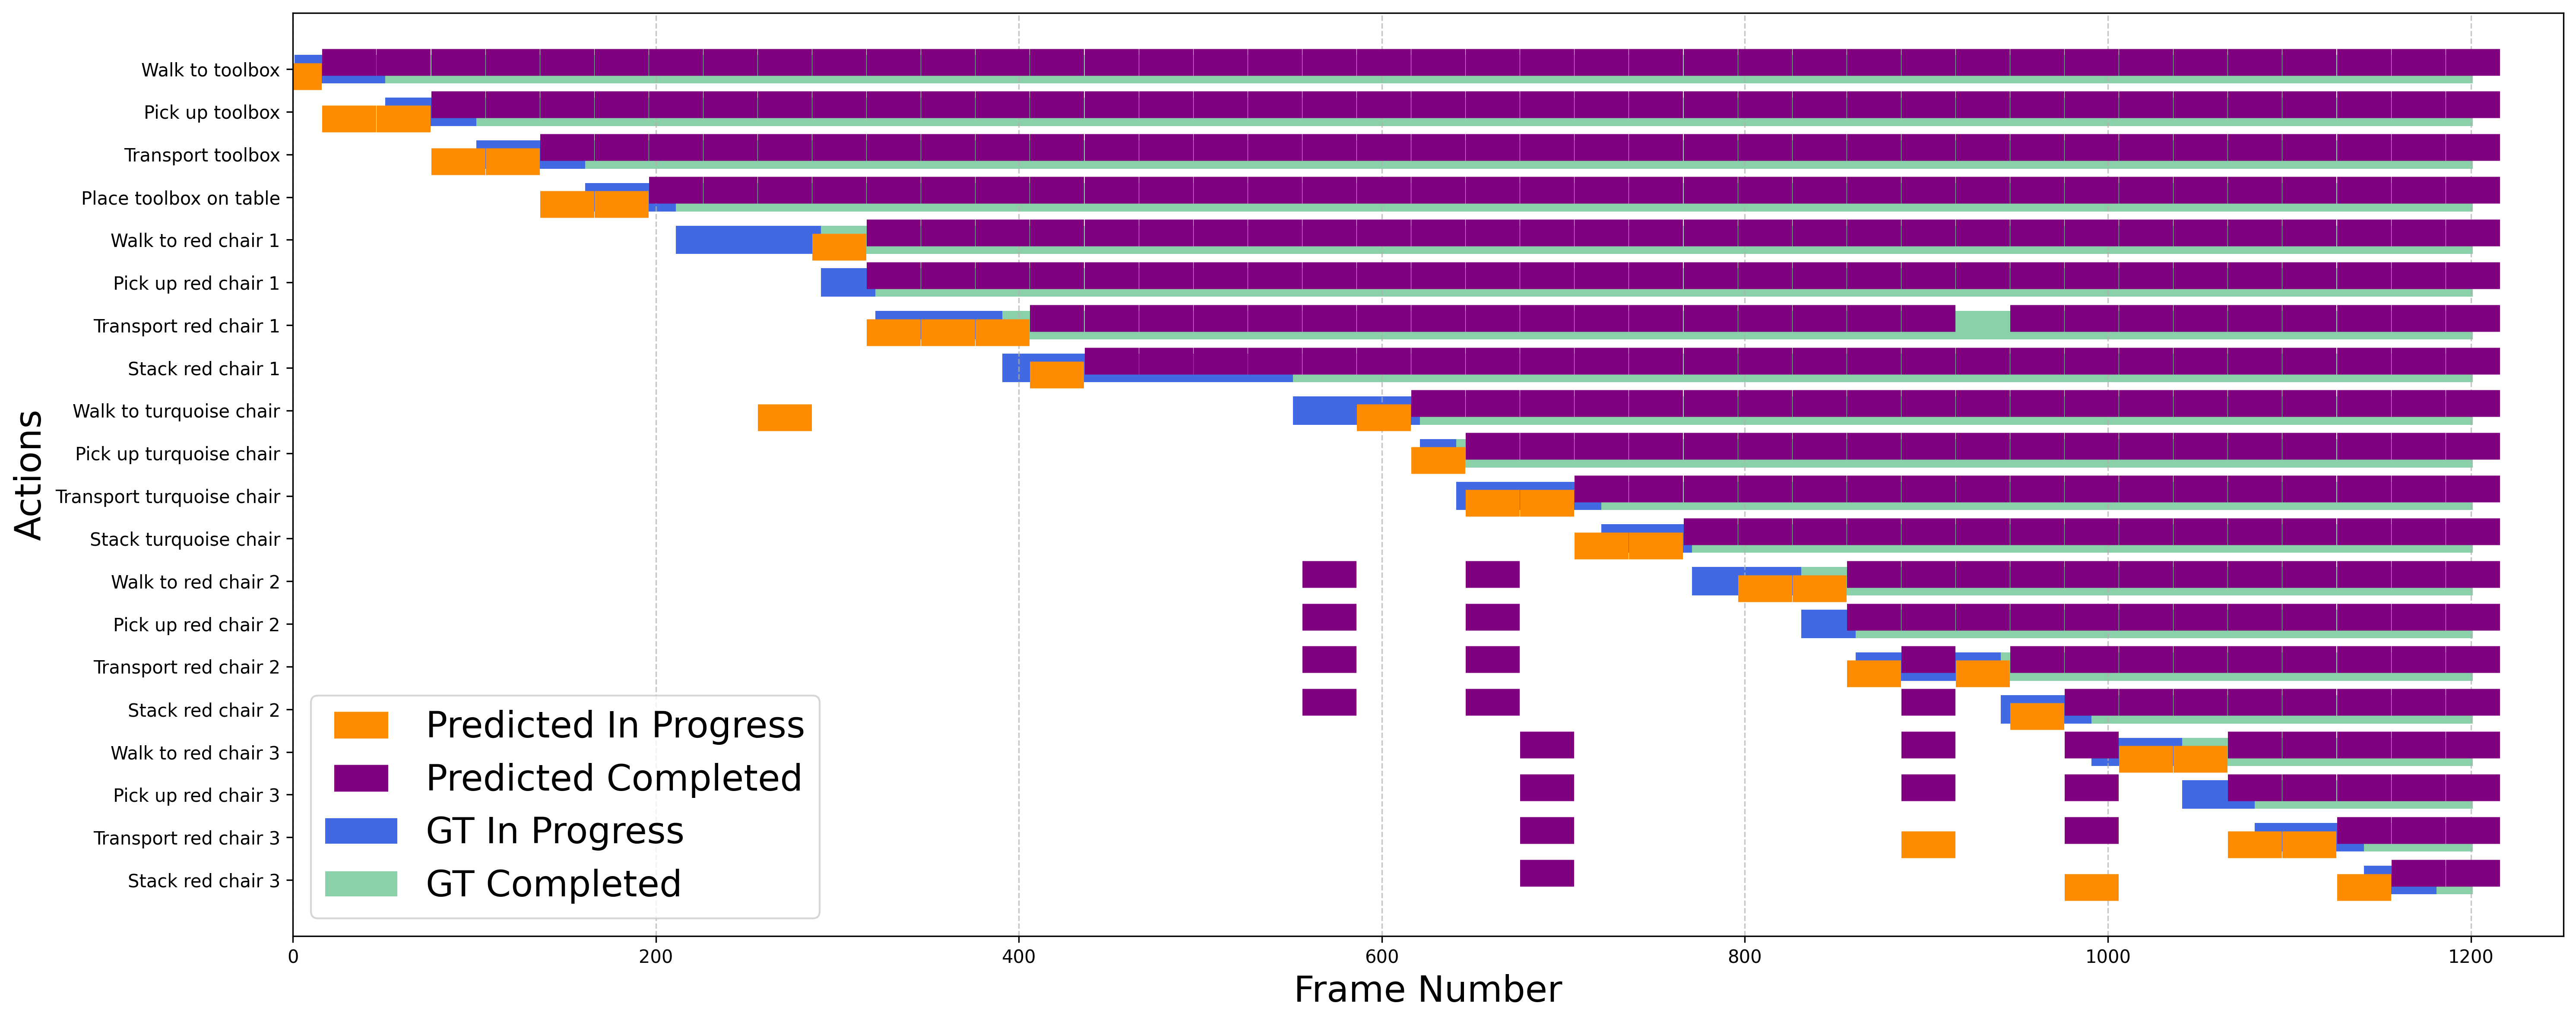
\includegraphics[width=1.3\textwidth, trim=0 0 0 25, clip]{ICL_Stack_gemini-2.5-pro_use_gaze_visualization.png}}
    \hfill
    \subfloat[][Use Case: Assembly]{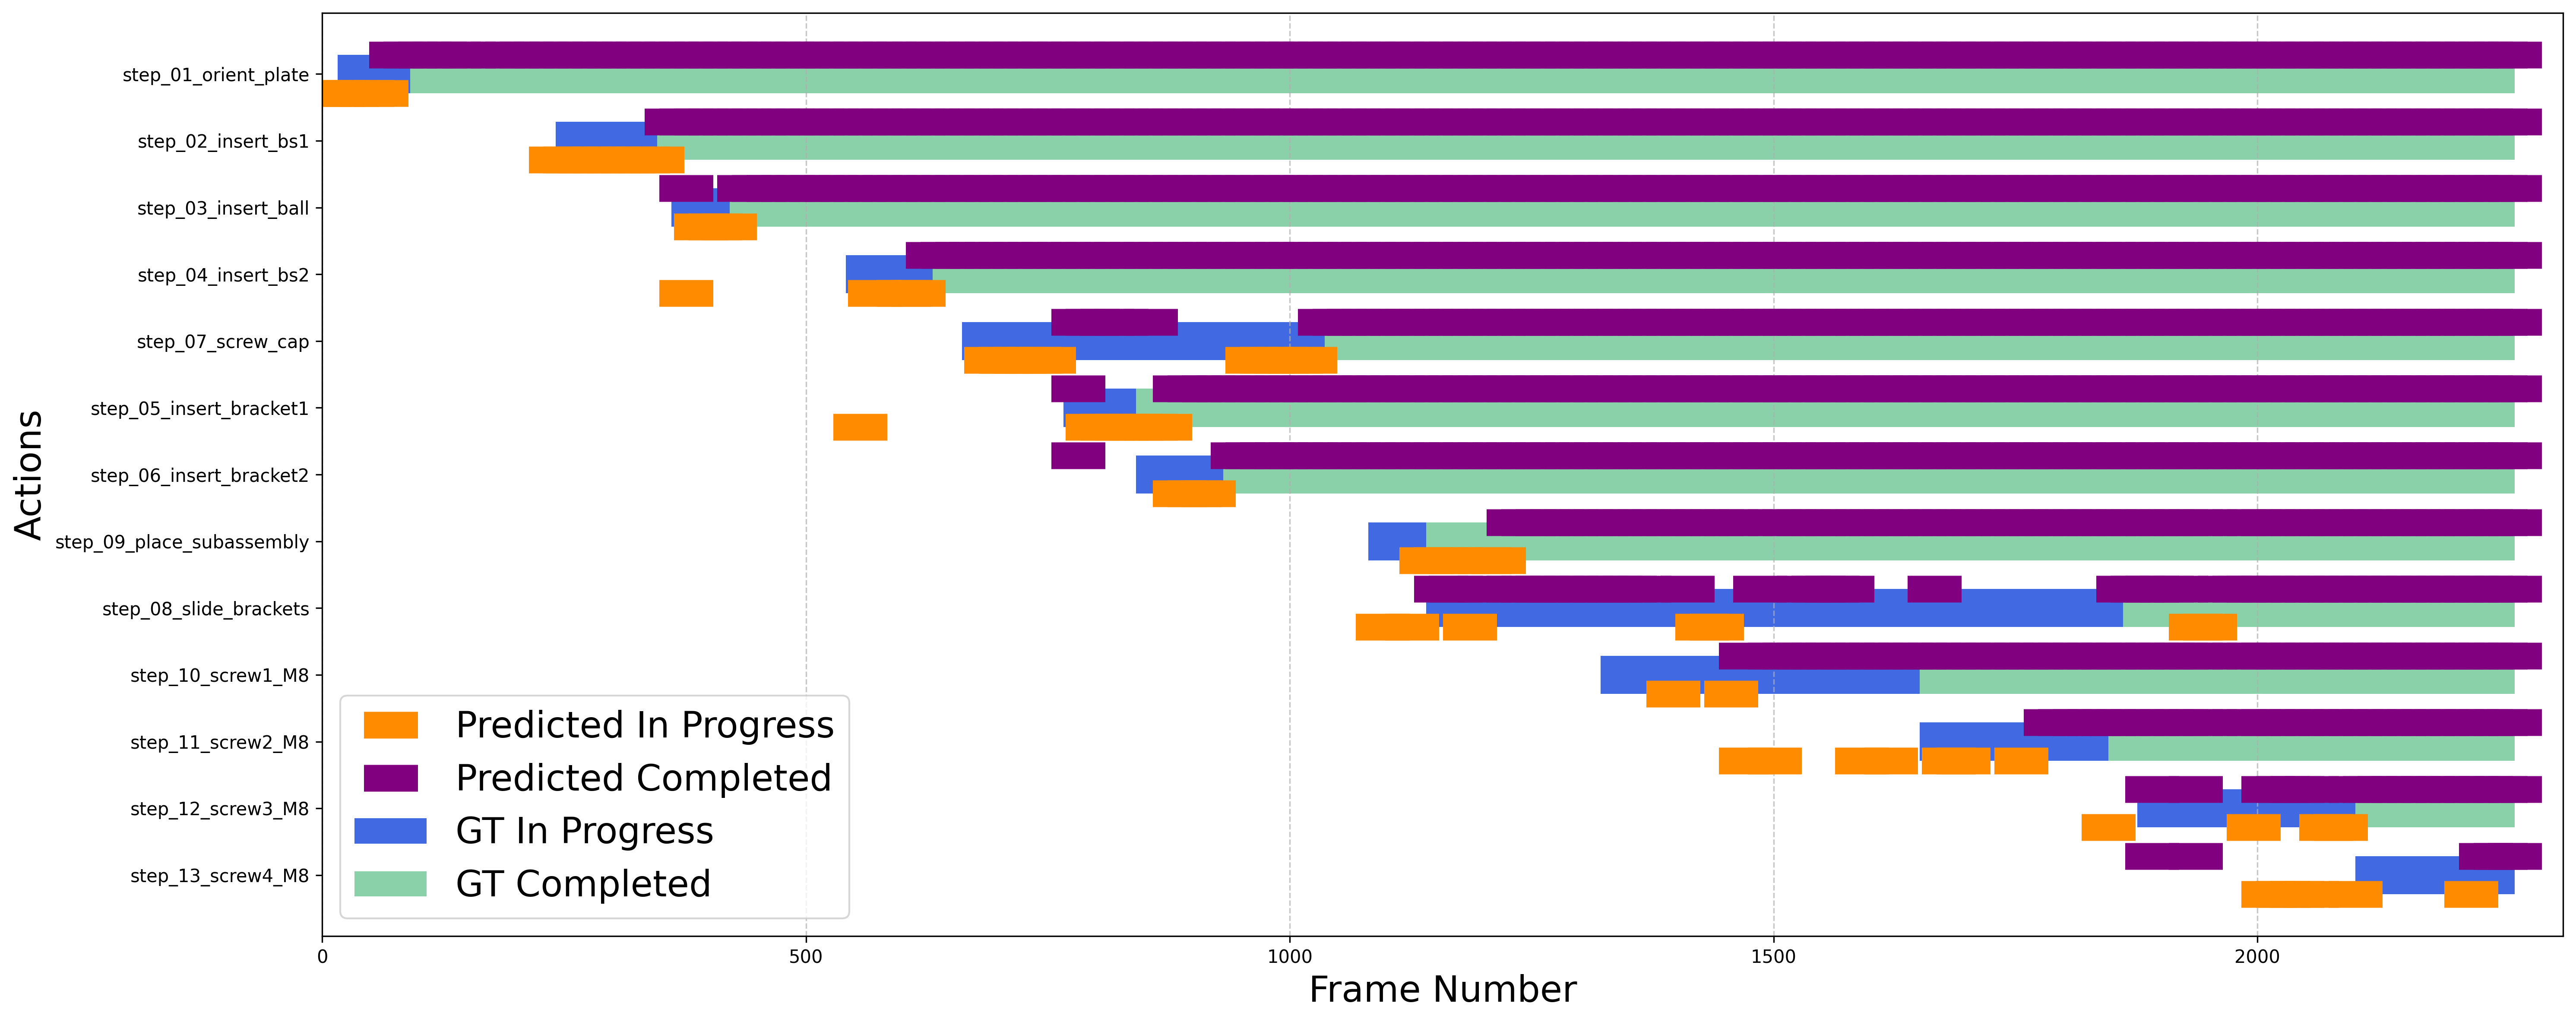
\includegraphics[width=1.3\textwidth, trim=0 0 0 25, clip]{RCWPS_HAViD_gemini-2.5-pro_no_gaze_use_gt_visualization.png}}
    \hfill
    \subfloat[][Use Case: Cooking]{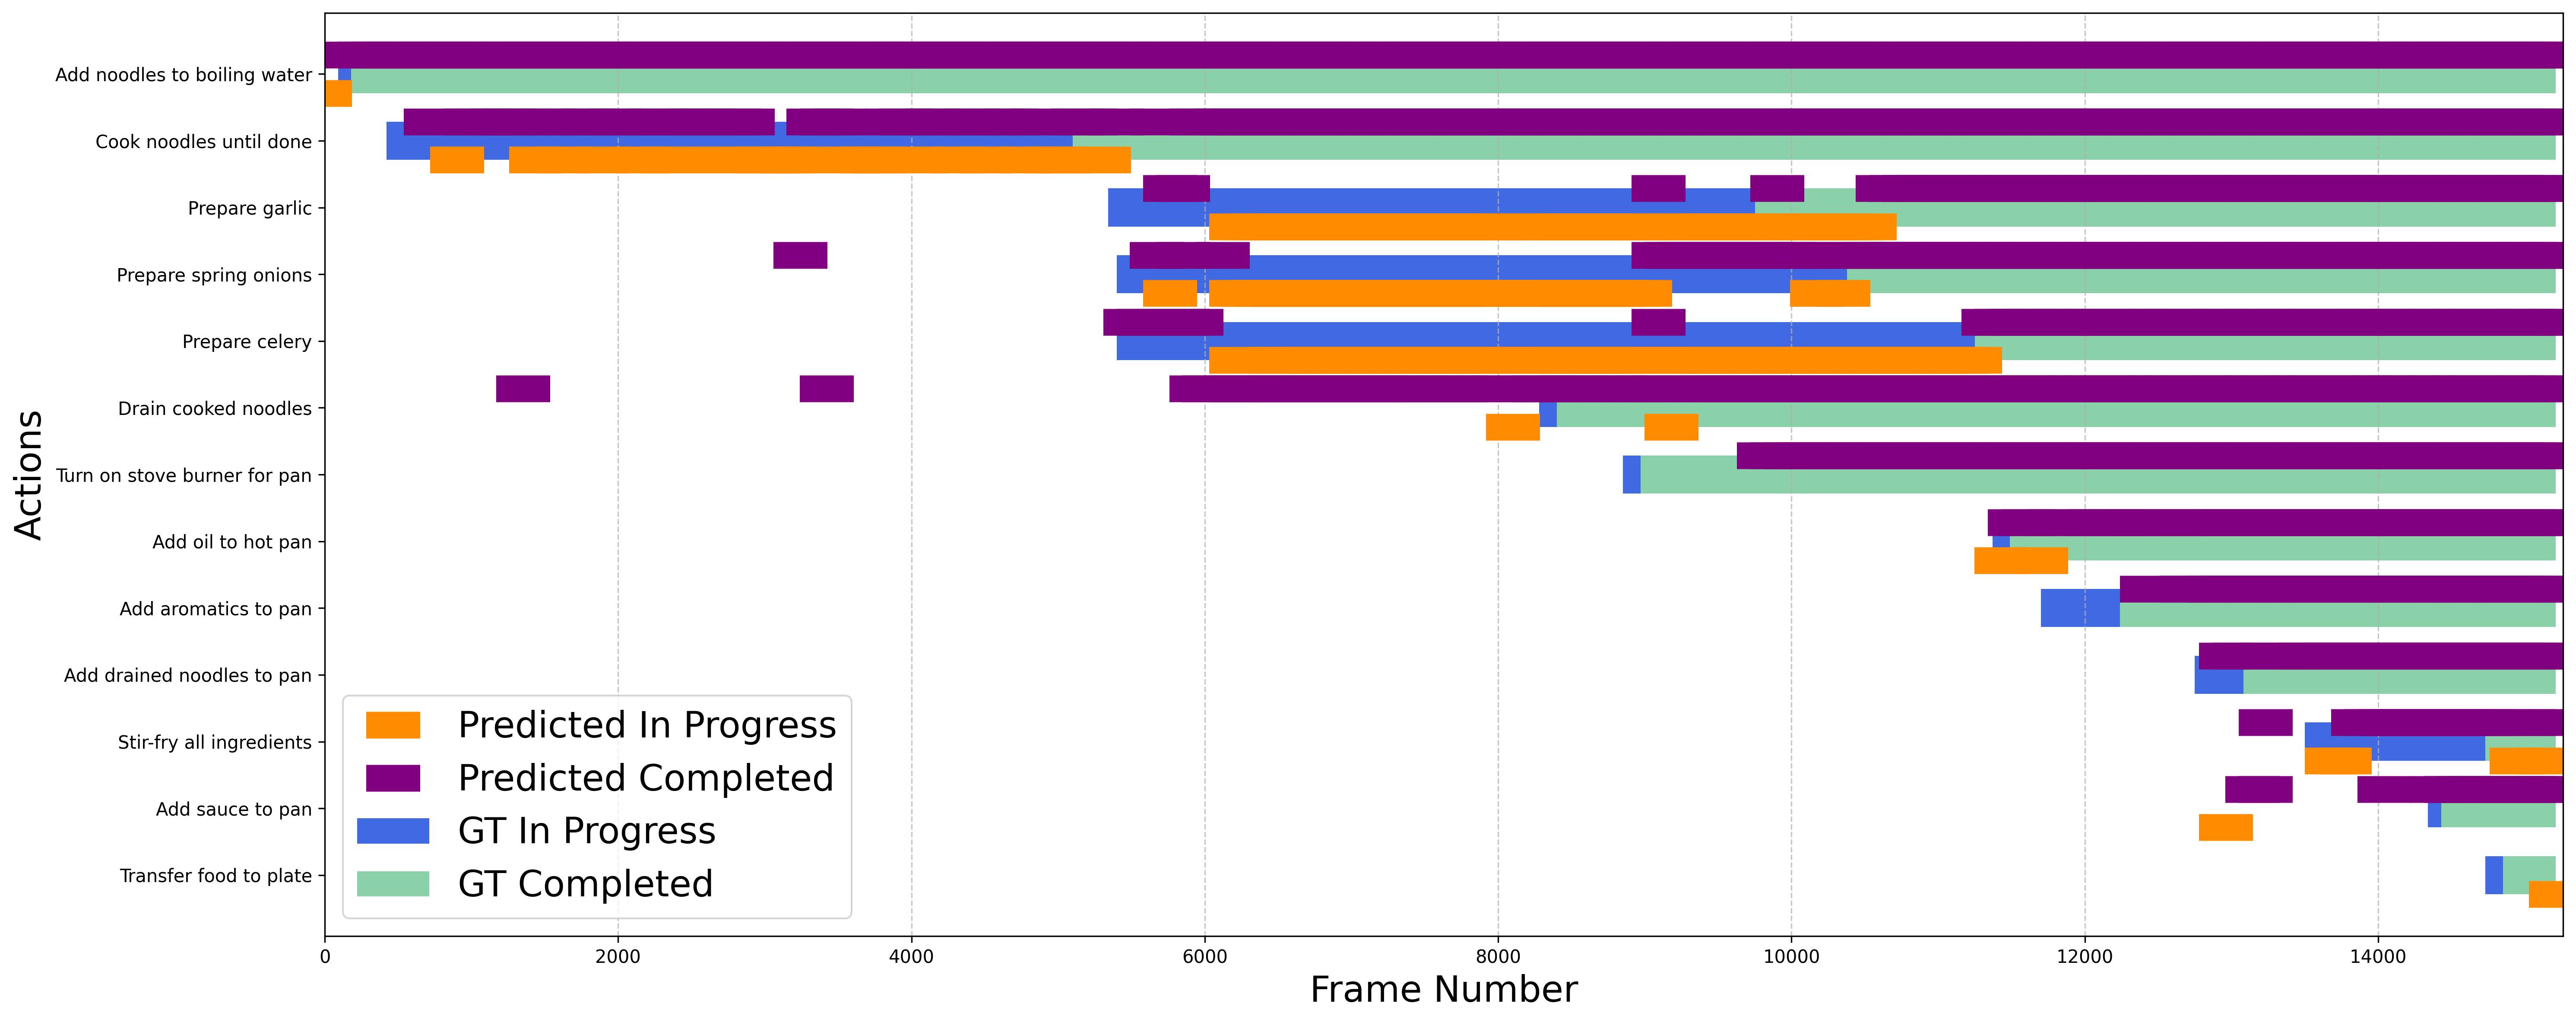
\includegraphics[width=1.3\textwidth, trim=0 0 0 25, clip]{RCWPS_Cooking_gemini-2.5-flash-lite_use_gaze_use_gt_use_ego_visualization.png}}
\end{adjustwidth}    
    \caption{Visualization of model performance across different use cases}
    \label{fig:timing_analysis}
\end{figure}


For the second phase, the prediction of future hand positions, the \textbf{Normalized Mean Position Error (NMPE)} is used. This metric calculates the average L2 norm (Euclidean distance) of the pixel error between the predicted and ground-truth hand coordinates, normalized from 0 to 1000.
\begin{linenomath}
\begin{equation}
    \text{NMPE} = \frac{1}{N} \sum_{i=1}^{N} \left( \frac{\sqrt{(x_{p,l} - x_{g,l})^2 + (y_{p,l} - y_{g,l})^2}_i + \sqrt{(x_{p,r} - x_{g,r})^2 + (y_{p,r} - y_{g,r})^2}_i}{2} \right)
\end{equation}
\end{linenomath}


where subscripts $p, g, l, r$ denote predicted, ground-truth, left hand, and right hand, respectively, for each prediction instance $i$ out of $N$.

While NMPE measures accuracy, it does not capture the exploratory nature of a model's predictions. A model that simply predicts minimal movement from the last known position might achieve a low NMPE but fail to anticipate significant, goal-directed actions. To quantify this, a \textbf{Prediction Diversity} metric is introduced. This metric measures how far a prediction deviates from the recent trajectory, rewarding predictions that are not mere extrapolations. It is calculated as the average of the Euclidean distances from the predicted point to both the average position and the final position of the hand in the input sequence, normalized by the standard deviation of the input positions.
\begin{linenomath}
\begin{equation}
\text{Diversity} = \frac{ D(\mathbf{p}_{\text{pred}}, \bar{\mathbf{p}}_{\text{in}})+  D(\mathbf{p}_{\text{pred}}, \mathbf{p}_{\text{last}})}{2\sqrt{\sigma(\mathbf{p}_{\text{in},x})^2 + \sigma(\mathbf{p}_{\text{in},y})^2}}
\end{equation}
\end{linenomath}
where $\mathbf{p}_{\text{pred}}$ is the predicted position, $\bar{\mathbf{p}}_{\text{in}}$ is the average position of the input trajectory, $\mathbf{p}_{\text{last}}$ is the last position in the input trajectory. Figure \ref{fig:error_analysis} shows the detailed error analysis for a sample Assembly scenario experiment.

\begin{figure}[h!]
    \centering       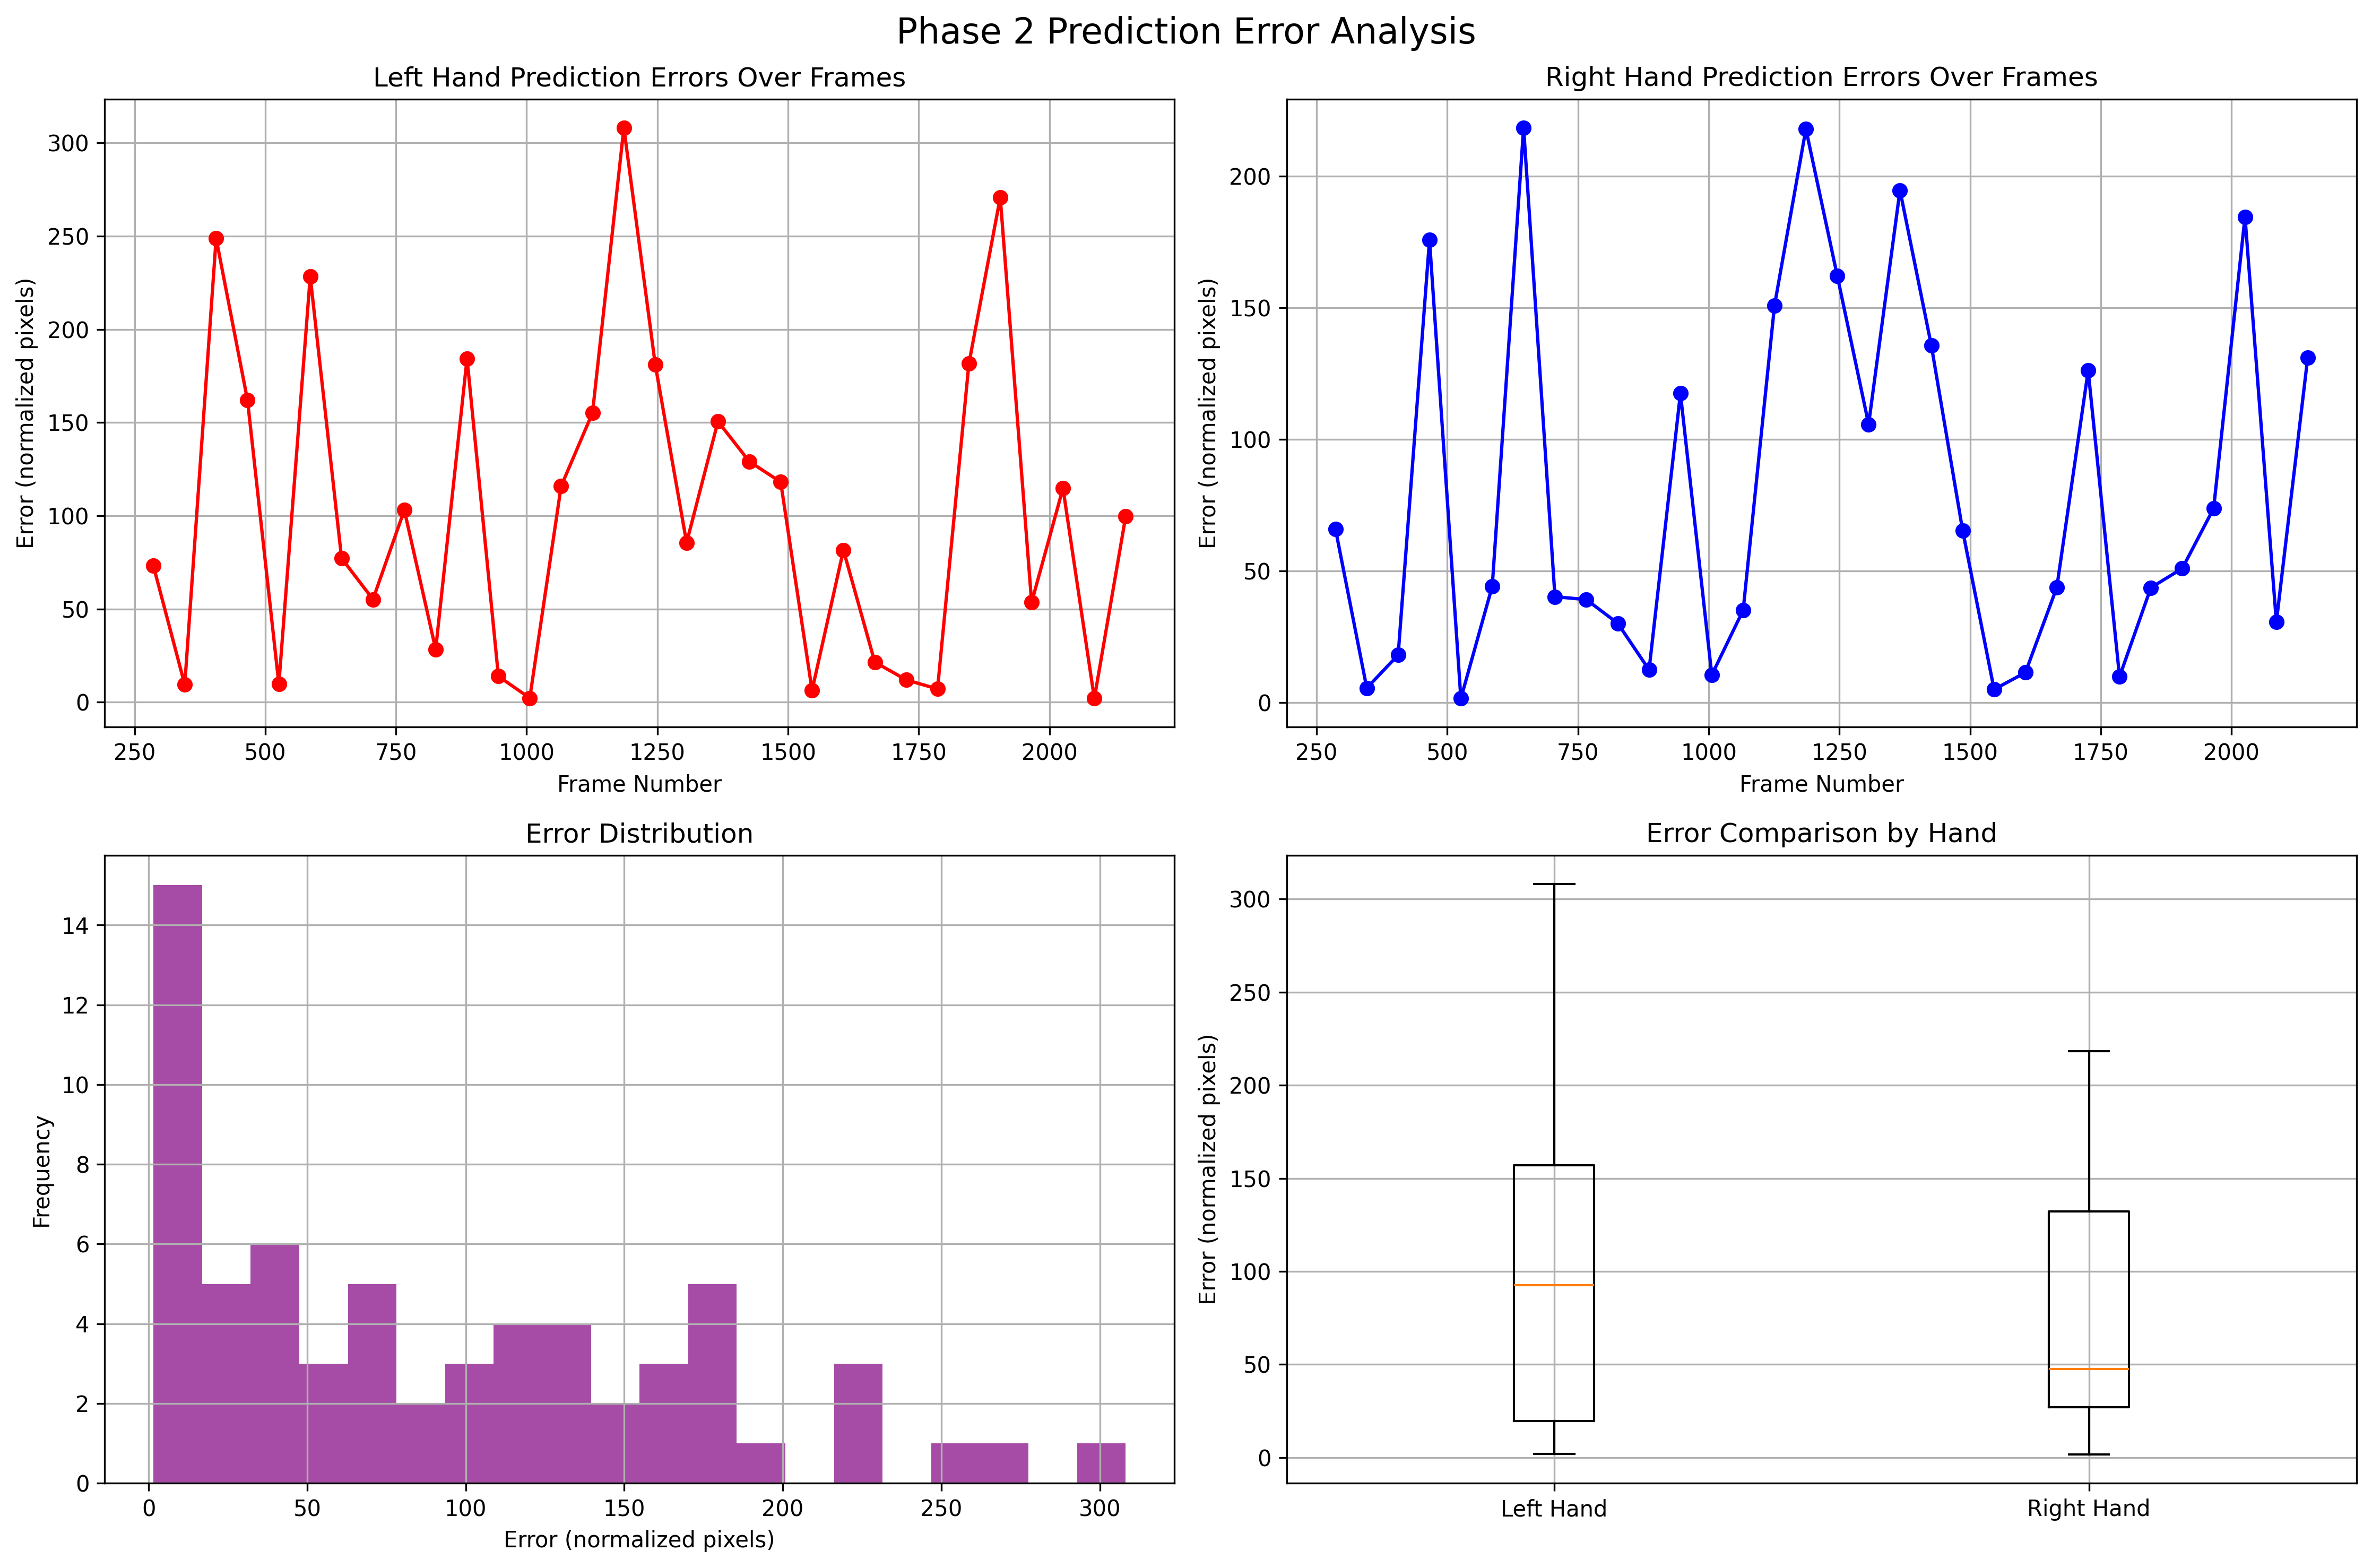
\includegraphics[width=\textwidth]{error_analysis.png} 
    \caption{Sample Error Analysis for hand position prediction for Assembly Scenario.}
    \label{fig:error_analysis}    
\end{figure}


\begin{table}[H]
\centering
\caption{Normalized Mean Position Error (NMPE) and Prediction Diversity by Use Case.}
\label{tab:nmpe_diversity_by_usecase}
\resizebox{\textwidth}{!}{%
\begin{tabular}{llccrr}
\toprule
\textbf{Use Case} & \textbf{Model} & \textbf{Gaze Data} & \textbf{Examples} & \textbf{NMPE} & \textbf{Diversity} \\
\midrule
\multirow{7}{*}{Stack} & Gemini 2.5 Flash Lite & Yes & 2-shot & 109.46 & 2.02 \\
& Gemini 2.5 Flash & Yes & 2-shot & 111.71 & 3.48 \\
& Gemma 3 27B & Yes & 0-shot & 114.97 & 2.33 \\
& Gemini 2.5 Flash Lite & No & 2-shot & 120.58 & 2.08 \\
& Gemini 2.5 Flash Lite & Yes & 0-shot & 121.74 & 1.42 \\
& Gemini 2.5 Pro & Yes & 2-shot & 152.68 & 5.68 \\
& Gemini 2.5 Pro & Yes & 1-shot & 181.76 & 6.14 \\
\midrule
\multirow{6}{*}{Assembly} & Gemma 3 27B  & N/A & 1-shot & 72.19 & 0.81 \\
& Gemini 2.5 Flash Lite & N/A & 2-shot & 74.70 & 1.20 \\
& Gemini 2.5 Flash Lite & N/A & 0-shot & 76.04 & 1.27 \\
& Gemini 2.5 Flash & N/A & 2-shot & 81.85 & 3.67 \\
& Gemini 2.5 Pro & N/A & 1-shot & 139.40 & 12.49 \\
& Gemini 2.5 Pro (No Context) & N/A & 0-shot & 202.35 & 23.05 \\
\midrule
\multirow{5}{*}{Cooking} & Gemini 2.5 Flash Lite & Yes & 0-shot & 70.16 & 1.04 \\
& Gemini 2.5 Flash Lite & Yes & 1-shot & 70.88 & 1.19 \\
& Gemini 2.5 Flash Lite & No & 1-shot & 74.49 & 1.31 \\
& Gemini 2.5 Flash & Yes & 2-shot & 78.36 & 2.69 \\
& Gemini 2.5 Pro & Yes & 1-shot & 89.34 & 3.37 \\
\bottomrule
\end{tabular}
}
\end{table}

\section{Discussion and Future Work}
\label{sec:discussion_conclusion}

The proposed modular framework advances the development of proactive robotic assistants by integrating state-of-the-art Vision-Language Models (VLMs) for high-level intent prediction with advanced models for perception and motion synthesis. This approach addresses key limitations in prior work. Unlike action recognition models that are confined to limited classes \citep{FutureTransformer, dexfocus} or context-agnostic pose forecasting methods \citep{STSGCN, transfusion}, our framework leverages the generalized reasoning capabilities of VLMs to interpret multi-modal context. 
By engineering this context through structured task graphs and rich perceptual data, the system can infer human intent in a way that is more aligned with the complexities of real-world tasks.

Prior work in social and assistive robotics often incorporates human intention within a narrow scope: to assess a user's engagement level \citep{Bi2023} or emotional state and respond appropriately \citep{Scassellati2002}. Such unstructured interactions do not involve completing a specific industrial task or adhering to formal Standard Operating Procedures (SOPs). In contrast, our framework is designed to predict task-based intentions within structured, goal-oriented workflows.

% \subsection{Limitations}
Despite its promise, the framework has several limitations that guide future research. The framework's current reliance on pre-defined task graphs, even when AI-assisted, restricts its applicability in completely unstructured or novel scenarios where a task plan is not available beforehand. Furthermore, the motion generation pipeline is not object-aware. While it utilizes the CLoSD model \citep{tevet2024closd} for physically plausible motion synthesis,the generated motions do not explicitly account for geometric interactions with specific objects in the environment. We address this limitation pragmatically by decoupling scene understanding from motion synthesis. The VLM, which is object-aware through its analysis of visual input, predicts a target 3D coordinate for a joint (e.g., placing a hand on a specific object). This 3D point then serves as a goal for the object-agnostic motion generation module. This approach functions as an effective workaround, but a fully integrated, object-aware motion model would be superior. Future work will explore integrating emerging models for physics-based human-object interaction with our modular framework. However, these methods often rely on datasets with a limited variety of objects and interactions \citep{intermimic, hot3d, arctic}. Finally, the use cases are centered on a single human operator, whereas many industrial environments involve complex multi-human collaborations, which introduce additional challenges such as occlusion and the need to interpret social dynamics.

% \subsection{Future Research Directions}
To address these limitations and expand the framework's capabilities, several avenues for future work are identified. A limitation of the current implementation is its reliance on a fixed-interval prediction cycle, where motion is forecast at regular time steps regardless of the task's dynamic context. Instead, an event-driven prediction framework can be explored where inference is triggered by salient cues, such as a sudden gaze shift or the completion of a task step. 

To improve generalization, methods for dynamically generating and adapting task graphs from observation may be explored, enabling the system to reason about unfamiliar workflows. Techniques inspired by multi-agent systems research \citep{magentic} could offer novel ways to coordinate the flow of information and aid decision-making. However, this approach is expected to add more latency to the system. Prompting strategies may be explored to encourage the VLM to recognize uncertainty and proactively seek clarification when its confidence is low or when critical information is missing, drawing inspiration from approaches like \citep{Chen2023}. Incorporating mechanisms for learning from human feedback or corrections during interaction \citep{Abeyruwan2022} could allow the system to be adaptable and responsive to task requirements and individual preferences. Further research can also explore the integration of additional context modalities, such as audio, physiological signals, or data from IoT sensors, to create a more holistic understanding of the operational environment. 

Another promising future direction is to use our framework’s proactive capabilities to enhance reactive impedance controllers for human-guided robots. By generating an anticipatory signal of where the user intends to move, an impedance controller can optimize its response in advance, rather than reacting solely to force. This would lead to a more symbiotic physical interaction with reduced human effort and improved task performance \citep{ImpedanceLearning}.

HCDTs powered by such human-centric situational awareness can serve as a virtual mentor for training, predict and flag ergonomically hazardous movements to prevent workplace injuries, or provide proactive robotic support by anticipating the need for assistance or carrying out tasks in parallel. Critically, the transition from research prototype to a practical industrial tool depends on rigorous real-world validation. Future work must involve deployment in real-time, lab-based HRC scenarios, where performance is assessed not only by prediction accuracy but also by HRC-centric metrics such as task efficiency, human idle time, and operator trust. Ultimately, this could enable a transition of robots from passive collaborative robots to intelligent coworkers.  

\section{Conclusion}
This paper presents a modular framework for context-aware human intent prediction and subsequent 3D motion generation, aimed at enabling proactive robotic assistance. By integrating pre-trained Vision Language Models with state-of-the-art perception and generation modules, the proposed approach provides a scalable solution that bridges high-level semantic reasoning with physically grounded motion synthesis. 

Our evaluation across three use cases of varying complexity revealed critical trade-offs between predictive accuracy, latency, and diversity. In-Context Learning (ICL) demonstrates notable limitations that counteract its potential benefits. The requirement for a large context token count results in significant computational latency and, in some cases, a paradoxical degradation of predictive accuracy, thus rendering the approach unsuitable for real-time applications. We identified the Rolling Context Window (RCW) strategy as a more viable approach, offering a strong balance of performance and efficiency. However, this method is susceptible to a consistency bias, where an initial error in state prediction can propagate and degrade subsequent performance. A key finding was that augmenting context with egocentric video views yielded a substantial 10.7\% performance increase in complex tasks.

Furthermore, in forecasting short-term motion, we observed a trade-off between accuracy and prediction diversity. More powerful models tended to generate predictions with higher diversity, attempting to forecast significant, goal-directed actions rather than simple extrapolations. This increased diversity, however, often came at the cost of higher position error. Additionally, predictive accuracy showed consistent improvement when providing one or two in-context examples (few-shot) compared to a zero-shot approach.


Through continued development and integration, the framework presented in this work can significantly advance the ability of robots to understand, anticipate, and effectively collaborate with humans in complex, dynamic settings.


%%%%%%%%%%%%%%%%%%%%%%%%%%%%%%%%%%%%%%%%%%
\vspace{6pt} 

%%%%%%%%%%%%%%%%%%%%%%%%%%%%%%%%%%%%%%%%%%
\authorcontributions{Conceptualization, U.A. and A.K.; methodology, U.A.; software, U.A.; validation, U.A., W.A.L and A.K.; investigation, U.A.; data curation, U.A.; writing—original draft preparation, U.A. and W.A.L; writing—review and editing, U.A., M.M.K., A.K., W.A.L. and S.R.; visualization, U.A.; supervision, M.M.K., A.K., W.A.L. and S.R.; project administration, M.M.K., A.K. and S.R. All authors have read and agreed to the published version of the manuscript.}

\funding{This research received no external funding.}

\institutionalreview{Not applicable.} 

\informedconsent{Informed consent was obtained from all subjects involved in the study. For the publicly available datasets (EgoExo4D and HA-ViD), the original data collectors were responsible for obtaining informed consent from the participants, and our study complies with the terms of use for these datasets. For the self-recorded data used in the Stacking scenario, one of the authors served as the subject and directly consented to participation.}

\dataavailability{Supplementary materials, videos, and the open-source implementation are available at the project website: \url{https://usmanasad88.github.io/hcdt/}}

\acknowledgments{The authors would like to acknowledge the Digital Innovation Research Group in the Department of Engineering at Nottingham Trent University, to support this work. The authors also like to thank developers of the open-source libraries and datasets used in this research.}

\conflictsofinterest{The authors declare no conflict of interest.} 

\abbreviations{Abbreviations}{
The following abbreviations are used in this manuscript:\\

\noindent 
\begin{tabular}{@{}ll}
AI & Artificial Intelligence \\
AR & Augmented Reality \\
BT & Behavior Tree \\
DAG & Directed Acyclic Graph \\
HCDT & Human-Centric Digital Twin \\
HMLV & High-Mix, Low-Volume \\
HRC & Human-Robot Collaboration \\
ICL & In-Context Learning \\
KG & Knowledge Graph \\
LLM & Large Language Model \\
ML & Machine Learning \\
MoCap & Motion Capture \\
NMPE & Normalized Mean Position Error \\
PDDL & Planning Domain Definition Language \\
POI & Point of Interest \\
RCW & Rolling Context Window \\
SME & Small and Medium Enterprises \\
SMPL-X & Skinned Multi-Person Linear Model with Extensions \\
TSA & Task State Accuracy \\
VLM & Vision-Language Model \\
VR & Virtual Reality
\end{tabular}
}

%%%%%%%%%%%%%%%%%%%%%%%%%%%%%%%%%%%%%%%%%%
% Citations and References in Supplementary files are permitted provided that they also appear in the reference list here. 
\begin{adjustwidth}{-\extralength}{0cm}
\reftitle{References}
\bibliography{export}

\PublishersNote{}
%\isPreprints{}{% This command is only used for ``preprints''.
\end{adjustwidth}

\end{document}